\documentclass[review]{elsarticle}
 
\usepackage{lineno,hyperref}
\modulolinenumbers[5]

\journal{Journal of \LaTeX\ Templates}

%%%%%%%%%%%%%%%%%%%%%%%
%% Elsevier bibliography styles
%%%%%%%%%%%%%%%%%%%%%%%
%% To change the style, put a % in front of the second line of the current style and
%% remove the % from the second line of the style you would like to use.
%%%%%%%%%%%%%%%%%%%%%%%

%% Numbered
%\bibliographystyle{model1-num-names}

%% Numbered without titles
%\bibliographystyle{model1a-num-names}

%% Harvard
%\bibliographystyle{model2-names.bst}\biboptions{authoryear}

%% Vancouver numbered
%\usepackage{numcompress}\bibliographystyle{model3-num-names}

%% Vancouver name/year
\usepackage{numcompress}\bibliographystyle{model4-names}\biboptions{authoryear}

%% APA style
%\bibliographystyle{model5-names}\biboptions{authoryear}

%% AMA style
%\usepackage{numcompress}\bibliographystyle{model6-num-names}

%% `Elsevier LaTeX' style
%\bibliographystyle{elsarticle-num}
%%%%%%%%%%%%%%%%%%%%%%%
\usepackage{xeCJK}
\usepackage{bm}
\usepackage{amsmath}
\usepackage{amssymb}
\usepackage{amsthm}
\usepackage{graphicx}
\usepackage{color}
\usepackage{booktabs}

\theoremstyle{plain}
\newtheorem{theorem}{\quad\quad Theorem}
\newtheorem{proposition}{\quad\quad Proposition}
\newtheorem{corollary}{\quad\quad Corollary}
\newtheorem{lemma}{\quad\quad Lemma}
\newtheorem{example}{Example}
\newtheorem{assumption}{\quad\quad Assumption}
\newtheorem{condition}{Condition}

\theoremstyle{definition}
\newtheorem{remark}{\quad\quad Remark}
\theoremstyle{remark}
\begin{document}

\begin{frontmatter}

\title{High-dimensional two-sample test under spiked covariance}

%% Group authors per affiliation:
    \author[mymainaddress]{Rui Wang}
    \author[mymainaddress,mysecondaryaddress]{Xingzhong Xu\corref{mycorrespondingauthor}}
\cortext[mycorrespondingauthor]{Corresponding author}
\ead{xuxz@bit.edu.cn}
    \address[mymainaddress]{School of Mathematics and Statistics, Beijing Institute of Technology, Beijing 
    100081,China}
    \address[mysecondaryaddress]{Beijing Key Laboratory on MCAACI, Beijing Institute of Technology, Beijing 100081,China}
%\fntext[myfootnote]{Since 1880.}

%% or include affiliations in footnotes:
%\author[mymainaddress,mysecondaryaddress]{Elsevier Inc}
%\ead[url]{www.elsevier.com}



\begin{abstract}
    This paper considers testing the means of two $p$-variate normal samples in high dimensional setting.  The covariance matrices are assumed to be spiked, which often arises in practice. 
    We propose a new test procedure through projection on the orthogonal complement of principal space.
    The asymptotic normality of the new test statistic is proved and the power function of the test is given.
    Theoretical and simulation results show that the new test outperforms existing methods substantially when the covariance matrices are spiked. Even when the covariance matrices are not spiked, the new test is acceptable.
\end{abstract}

\begin{keyword}
    high dimension, mean test, orthogonal complement of principal space, spiked covariance
\end{keyword}

\end{frontmatter}

%\linenumbers



\section{Introduction}

Suppose that $X_{k1},\ldots,X_{kn_k}$  are independent identically distributed (i.i.d.) as $N_p(\mu_k,\Sigma_k)$, where $\mu_k$ and $\Sigma_k$ are unknown, $k=1,2$. We consider the hypothesis testing problem:

\begin{equation}\label{problem}
    H_0:\mu_1=\mu_2\quad \textrm{vs.}\quad H_1:\mu_1\neq \mu_2.
\end{equation}
 In this paper, high dimensional setting is adopted, i.e., the dimension $p$ varies as $n$ increase, where $n=n_1+n_2$.
Testing hypotheses~\eqref{problem} is important in many applications, including biology, finance and economics. Quite often,  these data have strong correlations between variables. When strong correlations exist, covariance matrices are often spiked in the sense that a few eigenvalues are distinctively larger than the others. The paper is devoted to
testing hypotheses~\eqref{problem} in high dimensional setting with spiked covariance.


If $\Sigma_1=\Sigma_2=\Sigma$ is unknown, a classical test for hypotheses~\eqref{problem} is Hotelling's $T^2$ test.  Hotelling's test statistic is ${(\bar{X}_1-\bar{X}_2)}^T S^{-1}(\bar{X}_1-\bar{X}_2)$, where $S$ is the pooled sample covariance matrix. However, Hotelling's test is not defined when $p\geq n-1$.
Moreover,~\cite{Bai1996Efiect} showed that even if $p<n-1$, Hotelling's test suffers from low power when $p$ is comparable to $n$.
Perhaps, the main reason for low power of Hotelling's test is due to that $S$ is a poor estimator of $\Sigma$ when $p$ is large compared with $n$. See~\cite{Chen2010A} and the references therein.
In high dimensional setting,  
many test statistics in the literatures are based on an estimator of ${(\mu_1-\mu_2)}^T A(\mu_1-\mu_2)$ for a given positive definite matrix $A$. 
For example,~\cite{Bai1996Efiect} proposed a test based on
\begin{equation*}
    T_{BS}=\|\bar{X}_1-\bar{X}_2\|^2-(\frac{1}{n_1}+\frac{1}{n_2})\mathrm{tr}S,
\end{equation*}
which is an unbiased estimator of $\|\mu_1-\mu_2\|^2$.~\cite{Chen2010A} modified $T_{BS}$ by removing terms $\sum_{i=1}^{n_k}X_{ki}^T X_{ki}$, $k=1,2$ and proposed a test based on
\begin{equation*}
    \begin{aligned}
        T_{CQ}&=\frac{\sum_{i\neq j}^{n_1}X_{1i}^T X_{1j}}{n_1(n_1-1)}+\frac{\sum_{i\neq j}^{n_2}X_{2i}^T X_{2j}}{n_2(n_2-1)}-2\frac{\sum_{i=1}^{n_1}\sum_{j=1}^{n_2}X_{1i}^T X_{2j}}{n_1n_2}
        \\
            &=\|\bar{X}_1-\bar{X}_2\|^2-\frac{1}{n_1}\mathrm{tr}S_1-\frac{1}{n_2}\mathrm{tr}S_2,
    \end{aligned}
\end{equation*}
where $S_1$ and $S_2$ are sample covariance matrices. Statistic $T_{CQ}$ 
is also an unbiased estimator of $\|\mu_1-\mu_2\|^2$. Choosing $A={[\mathrm{diag}(\Sigma)]}^{-1}$,~\cite{Srivastava2008A} proposed a test based on
\begin{equation*}
    T_{S}={(\bar{X}_1-\bar{X}_2)}^T {[\mathrm{diag}(S)]}^{-1}(\bar{X}_1-\bar{X}_2),
\end{equation*}
where $\textrm{diag} (A)$ is a diagonal matrix with the same diagonal elements as $A$'s.
%To characterize strong correlation between variables,~\cite{Ma2015A} adopted a factor model proposed a test based on
%\begin{equation}\label{compete2}
 %    T_{FAST}=\frac{n_1 n_2}{n_1+n_2}\|\bar{X}_1-\bar{X}_2\|^2-(\mathrm{tr} S- \sum_{i=1}^{\hat{r}} \lambda_l(S))
%\end{equation}

As~\cite{Ma2015A} pointed out, however, these test procedures may not be valid if strong correlations exist, i.e., $\Sigma$ is far away from diagonal matrix. For example, the assumption 
%$$
%\mathrm{tr}(\Sigma_i \Sigma_j \Sigma_l \Sigma_h)=o[\mathrm{tr}^2\{{(\Sigma_1+\Sigma_2)}^2\}]\quad\quad  \textrm{for}\, i,j,l,h=1\,\textrm{or}\,2
%$$ 
\begin{equation}\label{chenscondition}
\mathrm{tr}(\Sigma^4)=o[\mathrm{tr}^2\{{(\Sigma)}^2\}]
\end{equation}
adopted by~\cite{Chen2010A} can be violated when $\Sigma=(1-c)I_p+c\bm{1}_p \bm{1}_p^T$ where $-{1}/{(p-1)}<c<1$, $I_p$ is the $p$ dimensional identity matrix and $\bm{1}_p$ is the $p$ dimensional vector  with elements $1$.
\cite{Ma2015A} considered a factor model and proposed a asymptotical parameter bootstrap procedure to adjust~\cite{Chen2010A}'s critical value.

Strong correlations between variables do exist in practice. In gene expression analysis, genes are correlated due to genetic regulatory networks (see~\cite{Thulin2014A}).~\cite{Chen2011A} pointed out that in terms of pathway analysis in proteomic studies,  test level can not be guaranteed if correlations are incorrectly assumed to be absent.
 As~\cite{Ma2015A} argued, there're strong correlations between different stock returns since they are all affected by the market index.

Incorrectly assuming the absence of correlation between variables will result in level inflation and low power for a test procedure. A class of test procedures is proposed through random projection (see~\cite{Lopes2015A},~\cite{Thulin2014A} and~\cite{Srivastava2014RAPTT}). The idea is to project data on some random lower-dimensional subspaces. It has been shown that these
procedures perform well under strong correlations. 

In many situations, the correlations are determined by a small number of factors.
Then $\Sigma$ is spiked (see~\cite{Cai2012Sparse}).
The random projection methods imply that test procedures are improved when data are projected on certain subspaces.
We will see that the ideal subspace is the orthogonal complement of the principal space.
Fortunately, the principal space can be estimated consistently even in high dimensional setting by the theory of principal component analysis (PCA).
%We find the ideal subspace is the orthogonal complement of the principal space.
%In this case, we know from the theory of principal component analysis (PCA) that the principal space can be estimated consistently even in high dimensional setting.
With the assumption of spiked covariance model, we propose a new test procedure through projection on the (estimated) ideal subspace.  
The asymptotic distribution of the test statistic is derived and hence asymptotic power is given.
%We will see that the asymptotic power function increases fast. In fact, the increasing rate is of a higher order than that of $T_{CQ}$.
We will see that the test is more powerful than $T_{CQ}$.
%Simulation study justifies the well-performance of the new test. Our theoretical results need the assumption $\sqrt{p}/(n_1+n_2)\to 0$. Simulation study shows that if it doesn't converge to $0$, the theorem may not be valid.
Moreover, even there's no strong correlation showing up, we prove that the new test performs equally well as $T_{CQ}$ does. The idea is also generalized to the unequal variance setting and similar results still hold.

%{\color{red}{To the best of our knowledge,~\cite{Ma2015A} and~\cite{2016arXiv160202491A} are the only work concerned on problem (~\eqref{problem}) when strong correlation exists.
%\cite{Ma2015A} adopted a factor model and modified the test statistic of~\cite{Chen2010A} to guarantee the test level. But we will see that the test still suffers from low power. In an independent working paper,~\cite{2016arXiv160202491A} adopted a spiked covariance structure, and their statistic is similar to ours. The main advantage of our work is that our theorems don't need strict relationship between $p$ and $n$. And our statistic is invariant under shift.
%}}


%{\color{red}{A fairly recent work~\cite{2016arXiv160202491A} proposed a new test for strongly spiked eigenvalue model. The proposed a test based on an estimation of
%\begin{equation}
%    \begin{aligned}
%        T_{AY}=&\frac{\sum_{i\neq j}^{n_1}X_{1i}^T\tilde{V}_1\tilde{V}_1^T X_{1j}}{n_1(n_1-1)}+\frac{\sum_{i\neq j}^{n_2}X_{2i}^T\tilde{V}_1\tilde{V}_1^T X_{2j}}{n_2(n_2-1)}
%        \\&-2\frac{\sum_{i=1}^{n_1}\sum_{j=1}^{n_2}X_{1i}^T\tilde{V}_1\tilde{V}_1^T\tilde{V}_2\tilde{V}_2^T X_{2j}}{n_1n_2}
%    \end{aligned}
%\end{equation}
%which is similar to our statistic in form. However, the theory framework is different. And we will see our statistic is different from theirs in some key properties.
%}}


The rest of the paper is organized as follows. In Section 2,  the model and some assumptions are given.  In Section 3, we propose a test procedure under $\Sigma_1=\Sigma_2$. Section 4 exploits properties of the test. In Section 5, we generalize our test procedure to the situation of $\Sigma_1\neq \Sigma_2$. In Section 6, simulations are carried out and  a real data example is given. Section 7 contains some discussion. All the technical details are in appendix.

\section{Model and assumptions}


Let $\{X_{k1},\ldots,X_{kn_k}\}$, $k=1, 2$ be two independent  random samples from $p$ dimensional normal distribution with means $\mu_1$ and $\mu_2$ respectively.

\begin{assumption}\label{balance}
Assume $p\to \infty$ as $n\to \infty$. Furthermore, assume two samples are balanced, that is,
\begin{equation*}
    \frac{n_1}{n_2}\to \xi \in (0,+\infty).
\end{equation*}
\end{assumption}

To characterize correlations between $p$ variables, we consider spiked covariance structure which is adopted by PCA study. See~\cite{Cai2012Sparse} and the references given there.
\begin{assumption}\label{theModel}
Suppose $X_{ki}$, $i=1,2,\ldots,n_k$ and $k=1,2$ are generated by  following model
\begin{equation*}
X_{ki}=\mu_k+V_k D_k U_{ki}+Z_{ki},
\end{equation*}
where
$U_{ki}$'s are i.i.d.\  random vectors distributed as $r_k$ dimensional standard normal distribution with $r_k$ fixed, 
$D_k=diag(\lambda_{k1}^{\frac{1}{2}},\ldots,\lambda_{k{r_k}}^{\frac{1}{2}})$ with $\lambda_{k1}\geq \cdots \geq \lambda_{k{r_k}}>0$,
$V_k$ is  a $p\times r_k$ orthonormal matrix, $Z_{ki}$'s are i.i.d.\ random vectors distributed as  $N_p(0,\sigma^2_k I_p)$ independent of $U_{ki}$'s and $\sigma^2_k>0$, $k=1,2$.
\end{assumption}
Then $X_{ki}\sim N(\mu_k,\Sigma_k)$, where $ 
\Sigma_k=\textrm{Var}(X_{ki})=V_k\Lambda_k V_k^T+\sigma^2_k I_p
$
, $\Lambda_k=D_k^2=diag(\lambda_{k1},\ldots,\lambda_{k{r_k}})$.
From Assumption~\ref{theModel}, $V_k V_k^T$ is the orthogonal projection matrix on the column space of $V_k$. Let $\tilde{V}_k$ be a $p\times (p-r_k)$ full column rank orthonormal matrix orthogonal to columns of  $V_k$.
%, that is $\tilde{V}_k^T V_k=O_{r_k\times(p-r_k )}$
 Note that $\tilde{V}_k$ may not be unique. But the projection matrix $\tilde{V}_k\tilde{V}_k^T$ is unique because $\tilde{V}_k\tilde{V}_k^T=I-V_k V_k^T$.


\begin{assumption}\label{orderOfBeta}
    Assume that there is some constant $\kappa>0$ and $\beta\geq \frac{1}{2}$ such that
    \begin{equation*}
        \kappa p^{\beta}\geq \lambda_{k1}\geq \cdots \geq\lambda_{kr_k}\geq \kappa^{-1}p^{\beta}.
\end{equation*}
\end{assumption}


The restriction $\beta\geq 1/2$ breaks down the Condition~\eqref{chenscondition}. If $\beta< 1/2$, Condition~\eqref{chenscondition} is meet and~\cite{Chen2010A}'s  method is valid. 
 Hence $\beta=1/2$ is the boundary of the scope between $T_{CQ}$ and our new test.
The case $\beta=1$ corresponds to the factor model in paper~\cite{Ma2015A} with some restrictions of parameters.


Finally, let $\tau={(n_1+n_2)}/{(n_1n_2)}$, $S$ be the pooled sample covariance.
\begin{equation}
S=\frac{1}{n-2}\sum_{k=1}^2\sum_{i=1}^{n_k} (X_{ki}-\bar{X}_k) {(X_{ki}-\bar{X}_k)}^T
    =\frac{(n_1-1)S_1+(n_2-1)S_2}{n-2},
\end{equation}
where
\begin{equation}
S_k=\frac{1}{n_k -1}\sum_{i=1}^{n_k} (X_{ki}-\bar{X}_k) {(X_{ki}-\bar{X}_k)}^T,
\end{equation}
is the sample covariance  of the sample $k$, $k=1,2$.


\section{Methodology}

In this section, we consider testing the hypotheses~\eqref{problem} with equal covariance matrices.
\begin{assumption}\label{theModel2}
Assume $V_1=V_2$, $D_1=D_2$, $\Lambda_1=\Lambda_2$, $\sigma_1=\sigma_2$ and $r_1=r_2$.
\end{assumption}

To simplify notations, the subscript $k$ of $\Sigma_k$, $V_k$, $D_k$, $\Lambda_k$, $\sigma_k$ and $r_k$ are dropped.
%\begin{equation}
%X_{ki}=\mu_k+V D U_{ki}+Z_{ki}.
%\end{equation}

\subsection{Motivation}
 %Facing a testing problem, a general pattern to derive a new test can be summarized as $3$ steps.
 %The first step is to propose a new statistic $T(X)$. 
 %Usually,  $T(X)$ is chosen to be an estimator of certain `distance' between null and alternative. $\mathrm{E}T=0$ under null and $\mathrm{E}T> 0$  under alternative.
 In high dimensional setting, many test procedures for hypotheses~\eqref{problem} is based on a statistic $T(X)$ which estimates ${(\mu_1-\mu_2)}^T A(\mu_1-\mu_2)$.
 Usually, $T(X)$ satisfies $\mathrm{E}T=0$ under null hypothesis and $\mathrm{E}T> 0$  under alternative.
 To determine the critical value, the asymptotic distribution of $T$ need to be derived, say 
 $$\frac{T-\textrm{E}T}{\sqrt{\textrm{Var}(T)}}\xrightarrow{\mathcal{L}} N(0,1).$$
 Since $\textrm{Var}(T)$ may depend on parameters, a ratio consistent estimator $\widehat{\textrm{Var}(T)}$ of $\textrm{Var}(T)$ is necessary. Then
 the rejection region of a level $\alpha$ test can be defined as $T(X)\geq \widehat{\textrm{Var}(T)}^{\frac{1}{2}}z_{1-\alpha}$ where $z_{1-\alpha}$ is the $1-\alpha$ quantile of $N(0,1)$. 
% Tests derived by the above pattern have an advantage in that it's clear what kind of alternatives the test favors. Many test procedures have been proposed for different $A$. In essence, test procedures for different $A$ are incomparable since they test different alternatives. For example, $T_{CQ}$ outperforms $T_S$ when $\Sigma$ is nearly an identity matrix. However, $T_S$ performs better when different variables are in different scales. 
%In general, it remains an important question that how to boost test power for a given `distance'.
The asymptotic power of the test is 
$$\Phi(\frac{\mathrm{E}T}{\sqrt{\mathrm{Var}(T)}}-z_{1-\alpha}).$$
Thus, a general idea to boost the power of test is to reduce the variance $\mathrm{Var}(T)$ while the mean $\mathrm{E}(T)$ varies relatively little.

Now we revisit $T_{BS}$ and $T_{CQ}$ which are both based on the estimation of $\|\mu_1-\mu_2\|^2$. Denote the spectral decomposition of $\Sigma$ by $\Sigma =\sum_{i=1}^p \lambda_i p_i p_i^T$  with $\lambda_1\geq \cdots \geq \lambda_p$, where $p_i$, $i=1,\ldots,p$, are orthonormal $p$ dimensional vectors. The main body of both $T_{BS}$ and $T_{CQ}$ is 
\begin{equation}\label{qifa}
    \frac{n_1 n_2}{n_1+n_2}\sum_{i=1}^p {(\bar{X}_1-\bar{X}_2)}^T  p_i p_i^T (\bar{X}_1-\bar{X}_2),
\end{equation}
which is a sum of $p$ independent terms. Since $\sqrt{{n_1 n_2}/{(n_1+n_2)}}(\bar{X}_1-\bar{X}_2)$ is distributed as $N(0,\Sigma)$, the variance of ${n_1 n_2}/{(n_1+n_2)} {(\bar{X}_1-\bar{X}_2)}^T  p_i p_i^T (\bar{X}_1-\bar{X}_2)$ is $2\lambda_i^2$ which decreases in $i$. By our previous argument, if a few leading terms with significantly large variance are removed, the modified test will be more powerful.


The argument is also supported by the likelihood ratio test. If $\Sigma$ is known, the LRT is based on 
\begin{equation}\label{qifafa}
    {(\bar{X}_1-\bar{X}_2)}^T\Sigma^{-1}(\bar{X}_1-\bar{X}_2)=\frac{n_1 n_2}{n_1+n_2}\sum_{i=1}^p \lambda_i^{-1}{(\bar{X}_1-\bar{X}_2)}^T  p_i p_i^T (\bar{X}_1-\bar{X}_2).
\end{equation}
The difference between~\eqref{qifa} and~\eqref{qifafa} is the weights $\lambda_i^{-1}$.
% For LRT, large $\lambda_i$'s corresponds to small weights in the sum.
%If $\lambda_i$ is large, then the corresponding term has a small weight $\lambda_i^{-1}$ in the sum. 
Unfortunately, $\lambda_i$'s are hard to precisely estimate in high dimensional setting. See~\cite{bai2010spectral} for detail. Nevertheless, it's possible to identify which $\lambda_i$'s are large. LRT implies the corresponding terms should have small weights, which coincides with our previous idea.
%If we assume there are correlations between $p$ variables, e.g. $\Sigma=(1-c)I+c\bm{1}_p \bm{1}_p^T$ where c is a constant fulfill $-\frac{1}{p-1}<c<1$, then $\frac{n_1 n_2}{n_1+n_2} {(\bar{X}_1-\bar{X}_2)}^T  p_1 p_1^T (\bar{X}_1-\bar{X}_2)$ distributed as $(cp+1-c)\chi^2_1$ whose variance is of order $p^2$ while $\frac{n_1 n_2}{n_1+n_2}\sum_{i=2}^p {(\bar{X}_1-\bar{X}_2)}^T  p_i p_i^T (\bar{X}_1-\bar{X}_2)$ is distributed as $(1-c)\chi^2_{p-1}$ whose variance is of order $p$. 
%The large variance is totally caused by term $p\chi^2_1$. 
%If we remove $\frac{n_1 n_2}{n_1+n_2} {(\bar{X}_1-\bar{X}_2)}^T  p_1 p_1^T (\bar{X}_1-\bar{X}_2)$ from $T_{BS}$, the variance of $T_{BS}$ can be significantly reduced to order $p$ from order $p^2$.

%Note that $\Sigma=(1-c)I+c\bm{1}_p+\bm{1}_p^T$ is just a special case of spiked covariance.

Under Assumption~\ref{theModel}, $\Sigma=V\Lambda V^T +\sigma^2 I_p$. The eigenvalues of $\Sigma$ are $\lambda_1+\sigma^2,\ldots,\lambda_r+\sigma^2,\sigma^2,\ldots,\sigma^2$. The eigenvectors corresponding to the first $r$ eigenvalues are columns of $V$. Follow our previous argument, if the principal subspace $VV^T$ is known, we project $X_{ki}$ on the orthogonal complement space $\tilde{V}\tilde{V}^T$ and invoke the statistic of~\cite{Chen2010A}. We define the following statistic

\begin{equation*}
\begin{aligned}
    T_{1}&=\|\tilde{V}^T(\bar{X}_1-\bar{X}_2)\|^2-\frac{1}{n_1}\mathrm{tr}(\tilde{V}^T S_1\tilde{V})-\frac{1}{n_2}\mathrm{tr}(\tilde{V}^T S_2\tilde{V}).
    \\
    %&=\frac{\sum_{i\neq j}^{n_1}X_{1i}^T\tilde{V}\tilde{V}^T X_{1j}}{n_1(n_1-1)}+\frac{\sum_{i\neq j}^{n_2}X_{2i}^T\tilde{V}\tilde{V}^T X_{2j}}{n_2(n_2-1)}-2\frac{\sum_{i=1}^{n_1}\sum_{j=1}^{n_2}X_{1i}^T\tilde{V}\tilde{V}^T X_{2j}}{n_1n_2}
\end{aligned}
\end{equation*}
the asymptotic normality of $T_1$ can be obtained by~\cite{Chen2010A}'s Theorem 1.

\begin{proposition}\label{oracleTheorem}
    Under Assumptions~\ref{balance}-\ref{theModel2} and local alternative, that means, $\frac{n}{p}\|\mu_1-\mu_2\|^2\to 0$, we have 
    \begin{equation*}
        \frac{T_1-\|\tilde{V}^T(\mu_1-\mu_2)\|^2}
        {\sigma^2\sqrt{2\tau^2 p}}\xrightarrow{\mathcal{L}}N(0,1).
    \end{equation*}
\end{proposition}

\begin{remark}
    The asymptotic variance of $T_1$ is of order $\tau^2 p$ while the asymptotic variance of $T_{CQ}$ is of order $\tau^2 p^{2\beta}$ by~\cite{Chen2010A}'s Theorem 1. The asymptotic variance is reduced significantly if $\beta>1/2$ and $p$ is sufficiently large.
\end{remark}

%\begin{remark}If $V$ is known, the model in Assumption~\ref{theModel} is very similar to random effects model. And our idea is just like REstricted Maximum Likelihood (REML).
%\end{remark}

%\begin{remark}
%    Suppose $\mu_1=\mu_2$. When $\beta>1/2$, the order of $T_1$'s variance is smaller than the order of $T_{CQ}$'s variance, which implies $T_1/(\sigma^2\sqrt{2\tau^2 p})$ is asymptotically independent of $T_{CQ}/\sqrt{2\tau^2 \mathrm{tr}\Sigma^2}$. Hence $T_1$ does provide additional information, although $T_1$ is inherited from $T_{CQ}$.  
%\end{remark} 


\subsection{New Test}
We denote by $\hat{V}$ and $\hat{\tilde{V}}$ the first $r$ and last $p-r$ eigenvectors of $S$ respectively.
Similarly, we denote by  $\hat{V}_i$ and $\hat{\tilde{V}}_i$ the first $r$ and last $p-r$ eigenvectors of $S_i$ respectively, $i=1,2$.
 As estimators of their population counterparts, these simple statistics actually reach the optimal convergence rate. See~\cite{Cai2012Sparse}.

Since $T_1$ depends on subspace $\tilde{V}\tilde{V}^T$ which is unknown, we must estimate it.
The first part of $T_1$ is $\|\tilde{V}^T (\bar{X}_1-\bar{X}_2)\|^2$.
We estimate it directly by $\|\hat{\tilde{V}}^T (\bar{X}_1-\bar{X}_2)\|^2$.
Note that the second part of $T_1$ is $\frac{1}{n_1}\mathrm{tr}(\tilde{V}^T S_1\tilde{V})$. Since it only involves sample one,
we estimate it by $\frac{1}{n_1}\mathrm{tr}(\hat{\tilde{V}}_1^T S_1\hat{\tilde{V}}_1)$. Similarly, we estimate the third part of $T_1$ by $\frac{1}{n_2}\mathrm{tr}(\hat{\tilde{V}}_2^T S_2\hat{\tilde{V}}_2)$.


%We are now in a position to propose a new statistic for testing the hypotheses~\eqref{problem}.
Define

\begin{equation*}
\begin{aligned}
    T_2&=\|\hat{\tilde{V}}^T(\bar{X}_1-\bar{X}_2)\|^2-\frac{1}{n_1}\mathrm{tr}(\hat{\tilde{V}}_1^T S_1\hat{\tilde{V}}_1)-\frac{1}{n_2}\mathrm{tr}(\hat{\tilde{V}}_2^T S_2\hat{\tilde{V}}_2).
    %T_2=\frac{\sum_{i\neq j}^{n_1}X_{1i}^T\hat{\tilde{V}}\hat{\tilde{V}}^T X_{1j}}{n_1(n_1-1)}+\frac{\sum_{i\neq j}^{n_2}X_{2i}^T\hat{\tilde{V}}\hat{\tilde{V}}^T X_{2j}}{n_2(n_2-1)}
%-2\frac{\sum_{i=1}^{n_1}\sum_{j=1}^{n_2}X_{1i}^T\hat{\tilde{V}}\hat{\tilde{V}}^T X_{2j}}{n_1n_2}
\end{aligned}
\end{equation*}
We propose our new test statistic as
\begin{equation}\label{myTest}
    Q=\frac{T_2}{\hat{\sigma}^2\sqrt{2\tau^2 p}},
\end{equation}
where $\hat{\sigma}^2$ is a ratio consistent estimator of $\sigma^2$. In next section, it will be proved that the asymptotic distribution under null of $Q$ is $N(0,1)$. We reject the null hypothesis when $Q$ is larger than the upper $\alpha$ quantile of $N(0,1)$.

\begin{remark}
    Compared with random projection method, our projection is determined by the structure of $S_1$, $S_2$ and $S$.
    We don't  project multiple times as random projection method did, which leads to reproducibility in practice.
\end{remark}


\begin{remark} The statistic $T_2$ is invariant under shift transformation, that is, $T_2$ is invariant when adding a vector to $X_{1i}$ and $X_{2j}$ simultaneously: $X_{1i}\mapsto X_{1i}+\mu$ and $X_{2j}\mapsto X_{2j}+\mu$, $i=1,\ldots,n_1$, $j=1,\ldots,n_2$.
\end{remark}


\begin{remark}
If $r$ is an unknown positive number, a consistent estimator of $r$ is
\begin{equation}\label{estimateR}
    \hat{r}=\textrm{argmax}_{l\leq R}\frac{\lambda_l(S)}{\lambda_{l+1}(S)},
\end{equation}
where $R$ is a hyperparameter. See~\cite{Ahn2009Eigenvalue} for detail. Therefore, without loss of generality, we will assume that $r$ is known.
%and deal with it saperately if $r=0$.
\end{remark}

    Theoretical results will show that the asymptotic variance of $T_2$ is significantly smaller than $T_{CQ}$. 
    On the other hand, the new test statistic estimates $\|\tilde{V}(\mu_1-\mu_2)\|^2$.
    Then the superiority of the new test will be established if 
    
\begin{equation}\label{yuedengyu}
    \frac{\|\tilde{V}(\mu_1-\mu_2)\|}{\|\mu_1-\mu_2\|}\approx 1.
\end{equation}
Unfortunately,~\eqref{yuedengyu}
is not always the case since there always exists some
$\tilde{V}$ and $\mu_1-\mu_2$ such that $\|\tilde{V}(\mu_1-\mu_2)\|=0$.
However,~\eqref{yuedengyu} is reasonable since $\tilde{V}\tilde{V}^T$ is nearly an identity matrix in the sense that
    ${\|I_p-\tilde{V}\tilde{V}^T\|_F^2}/{\|I_p\|_F^2}=r/p\to 0$. 
In bayesian framework, if we assume that the elements of $\mu_k$ are independently generated from certain probability distribution, it can be established that 
\begin{equation*}
    \frac{\|\tilde{V}(\mu_1-\mu_2)\|}{\|\mu_1-\mu_2\|}\xrightarrow{P}1.
\end{equation*}
Such assumption of $\mu_k$ will be used in Theorem~\ref{sameTheorem}.


In order to formulate a test procedure, $\sigma^2$ needs to be estimated.  Note that $\sigma^2$ can be written as
\begin{equation}\label{jjjVariance}
    \sigma^2=\sum_{i=r+1}^{p}\lambda_i(\Sigma).
\end{equation}
We estimate it by sample version:
\begin{equation*}
    \hat{\sigma}^2=\frac{1}{p-r}\sum_{i=r+1}^{p} \lambda_i(S).
\end{equation*}
If estimator $\hat{\sigma}^2$ of $\sigma^2$ is ratio consistent, the asymptotic distribution of~\eqref{myTest} will not change if we replace $\sigma^2$ by $\hat{\sigma}^2$  due to Slutsky's theorem.

%When $\frac{\sqrt{p}}{n_1+n_2}\to 0$, the critical value of our test can be approximated by it's asymptotic distribution which we will encounter later.
%However, it is a more practical issue to deal with the case when $n$ is small or the case when $p$ is much larger than $n$. In these cases, the null distribution is complicated and asymptotic distribution is a poor approximation of true distribution. Fortunately, permutation method can be used with the price of heavier computational burden. See~\cite{Lehmann}.



\section{Theoretical results}

In this section, we derive some properties of the new test statistic.


First we consider the case  when the eigenvalues of $\Sigma$ is bounded, i.e., there is no clear correlation between variables.
In many practical problems, the alternative is `dense', i.e., under $H_1$ the signals in $\mu_1-\mu_2$ spread out over a large number of co-ordinates. See~\cite{Tony2013}.
Similar to bayesian models, we assume a normal prior distribution for $\mu_k$ to characterize `dense' alternative.
When the eigenvalues of $\Sigma$ is bounded, spike variance model is not valid. Hence some estimators in our test procedure make no sense. Particularly, if  $\hat{r}$ is estimated by~\eqref{estimateR}. the $\hat{r}$ is nothing but a random integer not greater than $R$ and $\hat{V}\hat{V}^T$ is just a random projection. In this case, the difference of our test statistic and~\cite{Chen2010A}'s is small.
The next theorem shows that  the power of our new test is asymptotically the same as~\cite{Chen2010A}'s test in this case.


\begin{theorem}\label{sameTheorem}
   Assume $X_{ki}\sim N(\mu_k,\Sigma)$,  $i=1,\ldots,n_k$, $k=1,2$.
    Suppose that Assumptions~\ref{balance} and~\ref{pAndN} holds, $0<c\leq\lambda_p(\Sigma)\leq\lambda_1(\Sigma)\leq C<\infty$ where $c$ and $C$ are constants, each element of $\mu_k$ is independently generated by $N(0,{(n_k\sqrt{p})}^{-1}\psi)$ for $k=1,2$, where $\psi$ is a constant and  $\hat{r}$ is estimated by~\eqref{estimateR}.
    Then we have
    
\begin{equation*}
    \frac{T_2-\|\mu_1-\mu_2\|^2}{\sqrt{2\tau^2 \mathrm{tr}\Sigma^2}} \xrightarrow{\mathcal{L}} N(0,1).
\end{equation*}
\end{theorem}

\begin{theorem}\label{sameTheorem2}
    Under Assumptions~\ref{balance}-\ref{theModel2} with factor number $r=0$, if
    $$
    \|\mu_1-\mu_2\|^2=......,
    $$
    then
    $$
    \frac{T_2-\|\mu_1-\mu_2\|^2}{\sigma^2\sqrt{2\tau^2 p}}\xrightarrow{\mathcal{L}} N(0,1).
    $$
\end{theorem}
\begin{proof}[\textbf{Proof Of Theorem~\ref{sameTheorem2}}]
    Since $r=0$, $X_{ki}=\mu_k+Z_{ki}$, $i=1,\ldots,n_k$ and $k=1,2$.
    As in the proof of Theorem~\ref{sameTheorem}, we only need to prove
    $$
    \frac{\|\hat{\tilde{V}}^T(\bar{Z_1}-\bar{Z_2})+\hat{\tilde{V}}^T(\mu_1-\mu_2)\|^2-\|\mu_1-\mu_2\|^2-\tau p \sigma^2}{\sigma^2\sqrt{2\tau^2 p}}\xrightarrow{\mathcal{L}}N(0,1).
    $$
    Independent of data, generate a $p$ dimensional random orthogonal matrix with Haar invariant distribution.
\end{proof}

Now we establish the asymptotic normality of the new test statistic under spiked covariance model.
We first give a result of the convergence rate of $\hat{\sigma}^2$.
\begin{proposition}\label{varianceEstimation}
    Under Assumptions~\ref{balance}-\ref{theModel2}, we have that%      $\hat{\sigma}^2$ is consistent.
    $$
    \hat{\sigma}^2=\sigma^2 + O_P\Big(\frac{\max (n,p)}{np}\Big).
    $$
\end{proposition}
Proposition~\ref{varianceEstimation} implies that $\hat{\sigma}^2$ is a consistent estimator of $\sigma^2$.   

To derive the asymptotic normality of the new test statistic, we require the following relationship of $n$ and $p$.
\begin{assumption}\label{pAndN}
    Assume
    $
    {\sqrt{p}}/{n}\to 0.
    $
\end{assumption}

 


\begin{theorem}\label{myPanpan}
    Under Assumptions~\ref{balance}-\ref{pAndN},
if the local alternative holds, that is,
    $$\frac{n}{\sqrt{p}}\|\mu_1-\mu_2\|^2=O(1),$$
then 
\begin{equation*}
        \frac{T_2-\|\tilde{V}^T(\mu_1-\mu_2)\|^2}{\sigma^2\sqrt{2\tau^2 p}}\xrightarrow{\mathcal{L}}N(0,1).
\end{equation*}
\end{theorem} 
\begin{remark}
The Assumption~\ref{pAndN} is a strong condition.
However, it may not be able to relax it. In fact, the asymptotic normality of $T_2$'s main term $\|\hat{\tilde{V}}^T(\bar{X}_1-\bar{X}_2)\|^2$ requires 
\begin{equation}\label{eqREML}
    \frac{\lambda_1\big(\big(\hat{\tilde{V}}^T \Sigma \hat{\tilde{V}}\big)^2\big)}{\mathrm{tr}\big(\big(\hat{\tilde{V}}^T \Sigma \hat{\tilde{V}}\big)^2\big)
}\xrightarrow{P} 0,
\end{equation}
see Lemma~\ref{quadraticFormCLT} in appendix. And~\eqref{eqREML} is equivalent to Assumption~\ref{pAndN} by Lemma~\ref{conRateLemma} in appendix.
\end{remark}




%\begin{remark}  Compared with~\cite{2016arXiv160202491A}'s assumption (ix) which is equivalent to assuming $\frac{p^{2\beta-1}}{n_1+n_2}\to 0$ in model~\eqref{theModel}, our assumption $\frac{\sqrt{p}}{n_1+n_2}\to 0$ doesn't involved $\beta$.
%And when $\beta\geq \frac{3}{4}$, our assumption is weaker than~\cite{2016arXiv160202491A}'s. Note that when $\beta=\frac{1}{2}$, $\frac{\sqrt{p}}{n_1+n_2}$ is a necessary condition to make $\hat{V}\hat{V}^T$ a consistent
%estimator of $VV^T$ (see lemma 2 in appendix). So condition $\frac{\sqrt{p}}{n_1+n_2}$ is roughly the best we can do if the relationship between $p$ and $n$ doesn't involve $\beta$.
%\end{remark}

By Proposition~\ref{varianceEstimation}  and Theorem~\ref{myPanpan}, the power function of the new test can be obtained immediately.


\begin{corollary}\label{testPowerh}
    Under Assumptions~\ref{balance}-\ref{pAndN},
    if we reject the null hypothesis when $Q$ is larger than $1-\alpha$ quantile of $N(0,1)$, then the asymptotic power function of our test is
    \begin{equation*}
        \Phi\Big(-\Phi^{-1}(1-\alpha)+\frac{\|\tilde{V}(\mu_1-\mu_2)\|^2}{\sigma^2\sqrt{2\tau^2p}}\Big).
    \end{equation*}
\end{corollary}


 The power of $T_{CQ}$ is of the form
\begin{equation*}
    \Phi\Big(-\Phi^{-1}(1-\alpha)+\frac{\|\mu_1-\mu_2\|^2}{\sqrt{2\tau^2\mathrm{tr}\Sigma^2}}\Big).
\end{equation*}
 The relative efficiency of our test with respect to Chen's test is
\begin{equation*}
    \sqrt{\frac{\mathrm{tr}\Sigma^2}{(p-r)\sigma^4}}\frac{\|\tilde{V}(\mu_1-\mu_2)\|^2}{\|\mu_1-\mu_2\|^2}\sim p^{\beta-1/2}\frac{\|\tilde{V}(\mu_1-\mu_2)\|^2}{\|\mu_1-\mu_2\|^2},
\end{equation*}
which is large when $\beta>1/2$ and $\|\tilde{V}(\mu_1-\mu_2)\|/\|\mu_1-\mu_2\|$ is close to $1$.

When Assumption~\ref{pAndN} doesn't met, the asymptotic normality are not valid.
However, this does not mean the new statistic can not be used.
In fact, since the samples are exchangeable under null hypothesis, we can always use permutation method to determine the critical value.
We will see from simulation results that the new test has good power behavior even in large $p$ small $n$ case.


\section{Unequal Variance}

In this section, we concern the situation with unequal covariance matrices.
%With the theoretic work we have done, it's not hard to deal with general case, that is, $\Sigma_1$ and $\Sigma_2$ are both spiked but don't need to be equal.
Assume $\{X_{11},\ldots, X_{1n_1}\}$ and $\{X_{21},\ldots, X_{2n_2}\}$ are both generated from the model in Assumption~\ref{theModel}.
Denote by $\hat{V}_k$ the first $r_k$ eigenvectors of $S_k$ for $k=1,2$.
With a little abuse of notation, let $VV^T$ be the projection on the sum of column spaces of $V_1$ and $V_2$, that is,
\begin{equation*}
    VV^T =(V_1,V_2){\big({(V_1,V_2)}^T (V_1,V_2)\big)}^{+}{(V_1,V_2)}^T.
\end{equation*}
where $A^{+}$ is the Moore-Penrose inverse of a matrix A. Similarly, let $\hat{V}\hat{V}^T$ be the projection matrix on the sum of column spaces of $\hat{V}_1$ and $\hat{V}_2$.
 We define $\tilde{V}\tilde{V}^T=I_{p}-VV^T$ and $\hat{\tilde{V}}\hat{\tilde{V}}^T=I_{p}-\hat{V}\hat{V}^T$. 

The previous statistic can not be directly used
since the principal subspace is different for $X_{1i}$ and $X_{2j}$. The idea here is to remove all large variance terms from $T_{CQ}$ by projecting data on the space $\tilde{V}\tilde{V}^T$. Thus, we propose a new test statistic as
\begin{equation*}
\begin{aligned}
    T_3&=\|\hat{\tilde{V}}^T(\bar{X}_1-\bar{X}_2)\|^2-\frac{1}{n_1}\mathrm{tr}(\hat{\tilde{V}}_1^T S_1\hat{\tilde{V}}_1)-\frac{1}{n_2}\mathrm{tr}(\hat{\tilde{V}}_2^T S_2\hat{\tilde{V}}_2).
%    T_3=\frac{\sum_{i\neq j}^{n_1}X_{1i}^T\hat{\tilde{V}}\hat{\tilde{V}}^T X_{1j}}{n_1(n_1-1)}+\frac{\sum_{i\neq j}^{n_2}X_{2i}^T\hat{\tilde{V}}\hat{\tilde{V}}^T X_{2j}}{n_2(n_2-1)}
%    -2\frac{\sum_{i=1}^{n_1}\sum_{j=1}^{n_2}X_{1i}^T\hat{\tilde{V}}\hat{\tilde{V}}^T X_{2j}}{n_1n_2}
\end{aligned}
\end{equation*}


The theoretical results are parallel to those in equal variance setting.

%Compared with~\cite{2016arXiv160202491A}, our statistic have several advantages.
%First, our new statistic is invariance under transformation $X_{1i}\mapsto X_{1i}+\mu$ and $X_{2j}\mapsto X_{2j}+\mu$. So the null distribution of our test doesn't effected by $\mu$ and the test level can be guarenteed. 
%Second, our statistic doesn't rely on any single eigenvector of $\hat{V}$ but on the whole principal space $\hat{V}\hat{V}^T$. As a result, our statistic is uniquely defined. 
%Third, our statistic enjoys higher computation efficiency than~\cite{2016arXiv160202491A}'s method.

\begin{theorem}\label{myXiaopanpan}
    Under Assumptions~\ref{balance}-\ref{orderOfBeta} and~\ref{pAndN},
     if 
    $$\frac{n}{\sqrt{p}}\|\mu_1-\mu_2\|^2=O(1),$$
     then we have
\begin{equation*}
    \frac{T_3-\|\hat{\tilde{V}}^T(\mu_1-\mu_2)\|^2}{\sqrt{\sigma_n^2}}\xrightarrow{\mathcal{L}} N(0,1).
\end{equation*}
where
$\sigma_n^2=\frac{2(p-r_1-r_2)}{n_1(n_1-1)}\sigma_1^4+\frac{2(p-r_1-r_2)}{n_2(n_2-1)}\sigma_2^4+\frac{4(p-r_1-r_2)}{n_1n_2}\sigma_1^2\sigma_2^2$.
\end{theorem}
\begin{remark}
    Even if $\hat{\tilde{V}}_k\hat{\tilde{V}}_k^T$ is an consistent estimator of $\tilde{V}_k\tilde{V}_k^T$ for $k=1,2$, $\hat{\tilde{V}}\hat{\tilde{V}}^T$ may not be an consistent estimator of $\tilde{V}\tilde{V}^T$.
    Nevertheless, the asymptotic normality still holds.
    However, the centering term should be $\|\hat{\tilde{V}}^T(\mu_1-\mu_2)\|^2$ and can not be replaced by $\|\tilde{V}^T(\mu_1-\mu_2)\|^2$.
\end{remark}

 $\sigma_n^2$ can be estimated by ratio consistent estimators of $\sigma^2_k$ for $k=1,2$. Thus, if $n$ and $p$ are large and ${\sqrt{p}}/{n}$ is small, we reject when $T_3/\sqrt{\hat{\sigma}_n^2}>z_{1-\alpha}$. 
 %If $n$ is small or $p$ is large compared with n, we use permutation method to determine critical value.




\section{Numerical studies}
\subsection{Simulation results}

Our simulation study focus on equal variance case. 
We generate $X_{ki}$ by the model in Assumption~\ref{theModel}, where each element of $U_{ki}$ and $Z_{ki}$ are generated from $N(0,1)$.
$V$ is a random orthonormal matrix. 
We generate $\lambda_i$ as $p^{\beta}$ plus a random error from $U(0,1)$.

%The key to the validation of Theorem~\ref{myPanpan} is  that $T_{\textrm{dif}}=\frac{n_1n_2|T_1-T_2|}{\sqrt{2p}(n_1+n_2)\sigma^2}$ converges to $0$.
%Here we verify it by simulation.
%We set $n_1=n_2=n$, $p=n^i$ for $i=1,2$ and plot $T_{\textrm{dif}}$ versus $p$.
%The results are illustrated in figure~\ref{fig:fig1}.
%From the results we can find that $T_{\textrm{dif}}$ clearly converges to $0$ when $p=n$.
%In the case of $p=n^2$ which is exactly beyond the assumption of Theorem~\ref{myPanpan},
%$T_{\textrm{dif}}$ is large and it's not clear whether $T_{\textrm{dif}}$  converges to $0$.
%\begin{figure}
%    \centering 
%    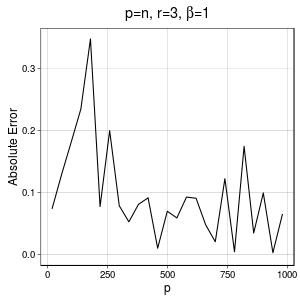
\includegraphics[height=6cm]{code/difference1.jpeg}
%    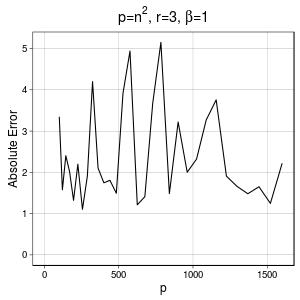
\includegraphics[height=6cm]{code/difference2.jpeg}\\
%    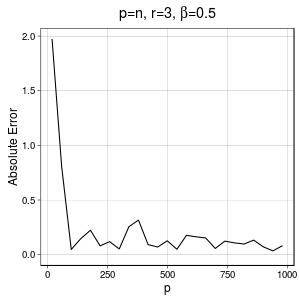
\includegraphics[height=6cm]{code/difference3.jpeg}
%    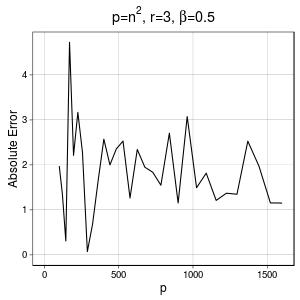
\includegraphics[height=6cm]{code/difference4.jpeg}\\
%    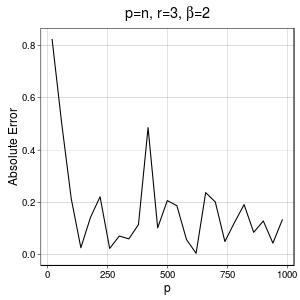
\includegraphics[height=6cm]{code/difference5.jpeg}
%    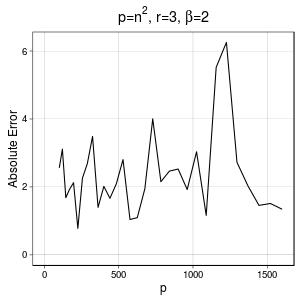
\includegraphics[height=6cm]{code/difference6.jpeg}\\
%    \caption{These are plots of $T_{\textrm{dif}}$ versus $p$. The first column and the second column are the case of $p=n$ and $p=n^2$, separately. The cases of $\beta=1,2,3$ are in the row $1,2,3$ separately. $r$ is set to be $3$ in all cases. }\label{fig:fig1}
%\end{figure}

First we simulate the level of the new test. The nominal level $\alpha=0.05$ and we set $r=2$. Samples are repeatedly generated $1000$ times to calculate empirical level.  For comparison, we also give corresponding `oracle' level which is calculated by `statistic' ${T_1}/(\sigma^2\sqrt{2p\tau^2})$ whose asymptotic normality can be guaranteed by Theorem 1 in~\cite{Chen2010A}. The results are listed in
Table~\ref{biaoge1}. From the results, we can find that for small $n$ and $p$, even oracle level is not satisfied. Level of the new test is  a little inflated compared with oracle level and it performs better when $n$ is larger.

% latex table generated in R 3.3.1 by xtable 1.8-2 package
% Sun Jul 31 01:50:20 2016
\begin{table}[ht]

\caption{Test level simulation} 
\label{biaoge1}
    \vspace{3mm}
\centering
\begin{tabular}{rccccccc}
    \toprule
     &  & \multicolumn{2}{c}{$\beta$=0.5} & \multicolumn{2}{c}{$\beta$=1}& \multicolumn{2}{c}{$\beta$=2}   \\
    \cmidrule(r){3-4}
    \cmidrule(r){5-6}
    \cmidrule(r){7-8}
$n$ & $p$ & NEW & ORACLE & NEW & ORACLE & NEW & ORACLE \\ 
\midrule
300 & 200 & 0.075 & 0.062 & 0.079 & 0.062 & 0.074 & 0.070 \\ 
  300 & 400 & 0.074 & 0.065 & 0.061 & 0.044 & 0.046 & 0.040 \\ 
  300 & 600 & 0.058 & 0.041 & 0.070 & 0.052 & 0.071 & 0.055 \\ 
  300 & 800 & 0.066 & 0.047 & 0.071 & 0.052 & 0.062 & 0.048 \\ 
  600 & 200 & 0.061 & 0.055 & 0.052 & 0.051 & 0.058 & 0.056 \\ 
  600 & 400 & 0.051 & 0.048 & 0.051 & 0.042 & 0.059 & 0.051 \\ 
  600 & 600 & 0.061 & 0.058 & 0.056 & 0.054 & 0.051 & 0.047 \\ 
  600 & 800 & 0.053 & 0.046 & 0.060 & 0.050 & 0.056 & 0.048 \\ 
   \bottomrule
\end{tabular}
\end{table}




Then we simulate the empirical power of our test and~\cite{Chen2010A}'s test. The simulation results of~\cite{Ma2015A} have showed that the level of the~\cite{Chen2010A}'s test can't be guaranteed when covariance is spiked. To be fair, we use permutation method to compute critical value. The validity of permutation method can be found in~\cite{Lehmann}'s Example 15.2.2. We plot the empirical power versus $\|\mu_1-\mu_2\|$ when other parameters hold constant. The results are illustrated in figure~\ref{fig:fig2}.
From the results, we can find that when $\Sigma$ is spiked, the new test outperforms $T_{CQ}$ substantially; when $\Sigma$ is not spiked, the new test and $T_{CQ}$ are comparable.
\begin{figure}
    \centering 
    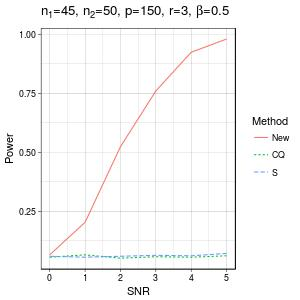
\includegraphics[height=6cm]{code/fig1.jpeg}
    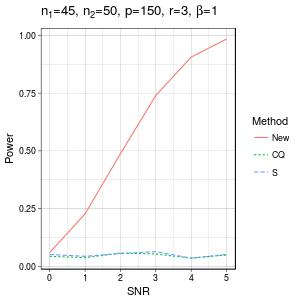
\includegraphics[height=6cm]{code/fig2.jpeg}
    \\
    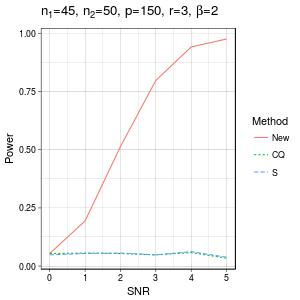
\includegraphics[height=6cm]{code/fig3.jpeg}
    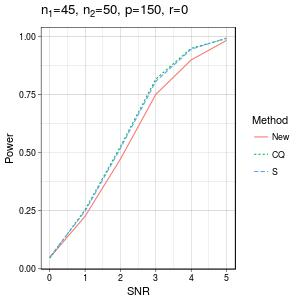
\includegraphics[height=6cm]{code/fig4.jpeg}
    \\
    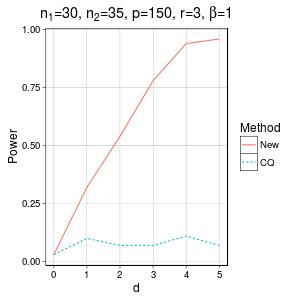
\includegraphics[height=6cm]{code/fig5.jpeg}
    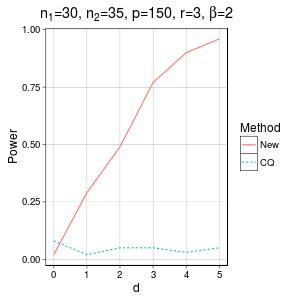
\includegraphics[height=6cm]{code/fig6.jpeg}
    \caption{Empirical power simulation. $\alpha$ is set to be $0.05$. $d$ is proportional to $\|\mu_1-\mu_2\|^2$. For each simulation, we do 50 permutations to determine critical value. We generate $100$ independent samples to compute empirical power. }\label{fig:fig2}
\end{figure}

%Permutation method is computation expensive. So when $p$ and $n$ are large, we simulate empirical power by asymptotic distribution. The results are illustrated in figure~\eqref{fig:fig3}.

%\begin{figure}\label{fig:fig3}
    %\centering 
    %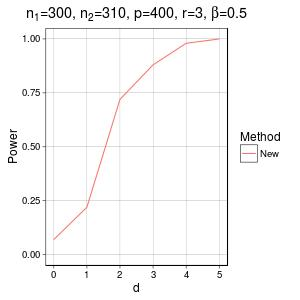
\includegraphics[height=6cm]{code/newfig1.jpeg}
    %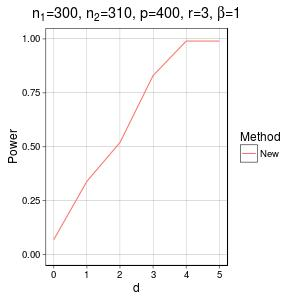
\includegraphics[height=6cm]{code/newfig2.jpeg}
    %\\
    %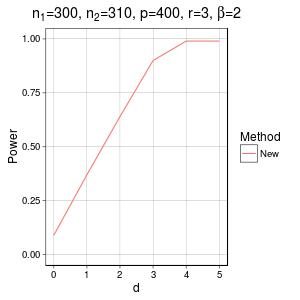
\includegraphics[height=6cm]{code/newfig3.jpeg}
    %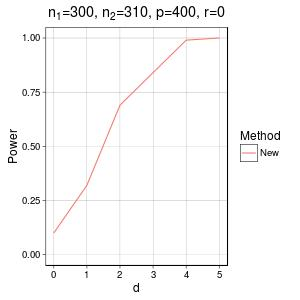
\includegraphics[height=6cm]{code/newfig4.jpeg}
    %\\
    %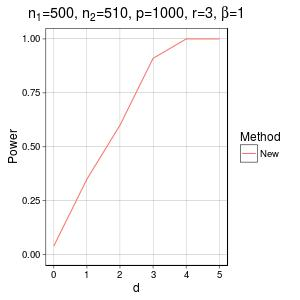
\includegraphics[height=6cm]{code/newfig5.jpeg}
    %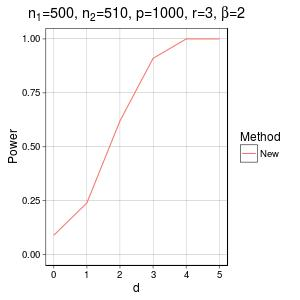
\includegraphics[height=6cm]{code/newfig6.jpeg}
    %\caption{Empirical Power (critical values are computed by asymptotic distribution)}\label{fig:fig3}
%\end{figure}

\subsection{Real data analysis}
In this section, we study the same practical problem as~\cite{Ma2015A} did. That is testing whether Monday stock returns are equal to those of other trading days on average. Define an observation be the log return of stocks in a day. Hence $p$ is the total number of stocks. Let sample $1$ and sample $2$ be the observations on Monday and the other trading days, respectively.  Then we would like to test $H_0\, :\mu_1=\mu_2$ v.s. $H_1\,:\mu_1\neq \mu_2$. We collected the data of $p=710$
 stocks of China
from 01/04/2013 to 12/31/2014. There are total $n_1=95$ Monday and $n_2=388$ other trading days. 

We assume $\Sigma_1=\Sigma_2$. The first eigenvaule of $S$ is $0.14$, which is significantly larger than the others.
In fact, the second eigenvalue is $0.02$.
Hence there's clearly a spiked eigenvalue. We set $r=1$ and perform our new test. The $p$ value is $0.149$, which is obtained by $1000$ permutations. Hence, the null hypothesis can not be rejected for $\alpha=0.05$. We draw the same conclusion as~\cite{Ma2015A}.

\section{Conclusion remark}

This paper is concerned with the problem of testing the equality of means in the setting of high dimension and spiked covariance. We removes big variance terms from $T_{CQ}$ and it's power is boosted substantially. The asymptotic normality of the new statistic is proved and the asymptotic power is given. %The new test outperforms $T_{CQ}$ substantially if the variance is spiked.
%We also generalize the test to unequal variance case.

In another paper,~\cite{Zhao2016A} proved their test statistic can be written in the form of projection. Their simulation results showed that their test performs well under strong correlations.
Our work partially explains why their test performs well although the projections are slightly different. 

 Spiked covariance is an important correlation pattern and has been widely studied in terms of PCA\@. In PCA, authors focus on the principal subspace. However, our work shows that in some circumstance, the complement of principal subspace is more useful. 


Our theoretical results rely on the assumption $\sqrt{p}/n\to 0$. In the situation of small sample or very large $p$, the critical value of the new test can be determined by permutation method. Our simulation shows that the new test still performs well. It remains a theoretical interest to study the asymptotic behavior of permutation based test in these situations.



\section*{Appendix}
We denote by $\|\cdot \|$ and $\|\cdot\|_F$ the operator and Frobenius  norm of matrix, separately.

%\begin{lemma}\label{lemma1}
%    let $X$ be a $p$-dimensional random vector with distribution $N(0,\Sigma)$. Denote the spectral decomposition of $\Sigma$ by $\Sigma =\sum_{i=1}^p \lambda_i p_i p_i^T$ with $\lambda_1\geq \cdots \geq \lambda_p$. Then $X^T p_i p_i^T X$ is stochastically larger than $X^T p_j p_{j}^T X$ for $i<j$.
%\end{lemma}
%\begin{proof}[\textbf{Proof}]
%    The lemma is established immediately once we note that $X^T p_i p_i^T X/\sqrt{\lambda_i}$ is distributed as $\chi^2$ distribution with freedom $1$.
%\end{proof}

\begin{lemma}[Weyl's inequality]
Let $H$ and $P$ be two symmetric matrices and $M=H+P$. If $j+k-n\geq i\geq r+s-1$, we have
\begin{equation*}
\lambda_j(H)+\lambda_k(P)\leq \lambda_i(M) \leq \lambda_r(H)+\lambda_s(P).
\end{equation*}
\end{lemma}
\begin{corollary}\label{WeylCor}
    Let $H$ and $P$ be two symmetric matrices and $M=H+P$. If $\mathrm{rank}(P)< k$, then
    \begin{equation*}
        \lambda_k(M)\leq \lambda_1(H).
    \end{equation*}
\end{corollary}


\begin{lemma}[Convergence rate of principal space estimation]\label{conRateLemma}
    Under the Assumption~\ref{balance}-\ref{theModel2}, we have
\begin{equation*}
E\|\hat{V}\hat{V}^T-VV^T\|^2_F =O(\frac{p}{p^{\beta}n}).
\end{equation*}
\end{lemma}


\begin{proof}[\textbf{Proof}]
    Theorem 5 of~\cite{Cai2012Sparse} asserts that sample principal subspace $\hat{V}\hat{V}^T$ is a minimax rate estimator of $VV^T$, namely, it reaches the minimax convergence rate
    \begin{equation}\label{xiaopianpian}
         E\|\hat{V}\hat{V}^T-VV^T\|^2_F\asymp r\wedge (p-r)\wedge \frac{r(p-r)}{(n_1+n_2-2)h(\lambda)}
    \end{equation}
    as long as the right hand side tends to $0$. Here $h(\lambda)=\frac{\lambda^2}{\lambda+1}$, $a_n\asymp b_n$ represents $a_n\geq cb_n$ and $a_n\leq Cb_n$ for some positive $c,C$ for every $n$. In model of Assumption~\ref{theModel},  $r$ is fixed, $\lambda=cp^\beta$.
    It's obvious that the right hand side of~\eqref{xiaopianpian} is of order ${p^{1-\beta}}/{n}$.
    We note that it is assumed $\beta\geq \frac{1}{2}$ in Assumption~\ref{orderOfBeta}, together with ${\sqrt{p}}/{n}\to 0$ we have
    ${p^{1-\beta}}/{n}\to 0$. Hence
    $\hat{V}\hat{V}^T$ reaches the convergence rate.

\end{proof}
\begin{lemma}[Bai-Yin's law]\label{baiyin}
    Suppose $B_n=\frac{1}{q} Z Z^T$ where $Z$ is $p\times q$ random matrix composed of i.i.d.\ random variables with zero mean, unit variance and finite fourth moment.
    As $q\to \infty$ and $\frac{p}{q}\to c\in [0,\infty)$, the largest and smallest non-zero eigenvalues of $B_n$ converge almost surely to ${(1+\sqrt{c})}^2$ and $(1-\sqrt{c})^2$, respectively.
\end{lemma}
\begin{remark}
    Lemma~\ref{baiyin} is known as the Bai-Yin's law (\cite{bai1993limit}). As in Remark $1$ of~\cite{bai1993limit}, the smallest non-zero eigenvalue is the $p-q+1$ smallest eigenvalue of $B$ for $c>1$.
\end{remark}
\begin{corollary}\label{maxEigen}
    Suppose that $W_n$ is a $p \times p$ matrix distributed as $\mathrm{Wishart}_p(n,I_{p})$. Then as $n\to \infty$,
    $$
        \lambda_1(W_n)=O_P(\max(n,p)).
    $$
\end{corollary}
\begin{proof}[\textbf{Proof}]
    Since $[0,+\infty]$ is compact, for every subsequance $\{n_{k}\}$ of $\{n\}$, there is a further subsequance $\{n_{k_l}\}$ along which $p/n\to c\in [0,+\infty]$.

    If $c\in [0,+\infty)$, by Lemma~\ref{baiyin}, we have that
    $$
    \frac{\lambda_1(W_{n_{k_l}})}{n_{k_l}}\xrightarrow{P}{(1+c)}^2.
    $$
    Hence the conclusion holds along this subsequance. If $c=+\infty$, suppose $W_n=Z_n Z_n^T$ where $Z_n$ is a $p\times n$ matrix with all elements distributed as $N(0,1)$. Then
    $$
    \frac{\lambda_1(W_{n_{k_l}})}{p}=\frac{Z_{n_{k_l}}^T Z_{n_{k_l}}}{p}\xrightarrow{P} 1,
    $$
    by Lemma~\ref{baiyin}, which proves the conclusion along the subsequance. Now the conclusion holds by a standard subsequance argument.
\end{proof}


\begin{lemma}\label{quadraticFormCLT}
    Suppose $X_{n}$ is a $k_n$ dimensional standard normal random vector and $A_n$ is a $k_n\times k_n$ symmetric matrix. Then a necessary and sufficient condition for
    \begin{equation}\label{quadratic}
        \frac{X_n^T A_n X_n-\mathrm{E}X_n^T A_n X_n}{{[\mathrm{Var}(X_n^T A_n X_n)]}^{1/2}}\xrightarrow{\mathcal{L}}N(0,1)
    \end{equation}
    is that
    \begin{equation}\label{quadraticEigen}
        \frac{\lambda_{\max}(A_n^2)}{\mathrm{tr}(A_n^2)}\to 0.
    \end{equation}
\end{lemma}
\begin{remark}
This lemma is from the Example 5.1 of~\cite{jiang1996reml}. Here we give a proof by characteristic function.
\end{remark}
\begin{proof}
    Let $\lambda_1(A_n)\geq\cdots\geq \lambda_{k_n}(A_n)$ be the eigenvalues of $A_n$, then 
    \begin{equation}
        \frac{X_n^T A_n X_n-\mathrm{E}X_n^T A_n X_n}{{[\mathrm{Var}(X_n^T A_n X_n)]}^{1/2}}=\sum_{i=1}^{k_n}\frac{\lambda_i(A_n)}{{\big[2\mathrm{tr}(A_n^2)\big]}^{1/2}}(Z_{ni}^2-1),
    \end{equation}
    where $Z_{ni}$'s ($i=1,\ldots,k_n$) are independent standard normal random variables.

    If~\ref{quadraticEigen} holds, then
    \begin{equation*}
        \begin{aligned}
            &\sum_{i=1}^{k_n}\mathrm{E}\Big[\frac{\lambda_i^2(A_n)}{2\mathrm{tr}(A_n^2)}{(Z_{ni}^2-1)}^2\Big\{\frac{\lambda_i^2(A_n)}{2\mathrm{tr}(A_n^2)}{(Z_{ni}^2-1)}^2\geq \epsilon\Big\}\Big]\\
            \leq&\sum_{i=1}^{k_n}
            \frac{\lambda_i^2(A_n)}{2\mathrm{tr}(A_n^2)}
            \mathrm{E}\Big[{(Z_{n1}^2-1)}^2\Big\{\frac{\lambda_{\max}(A_n^2)}{2\mathrm{tr}(A_n^2)}{(Z_{n1}^2-1)}^2\geq \epsilon\Big\}\Big]\\
            =&
            \frac{1}{2}\mathrm{E}\Big[{(Z_{n1}^2-1)}^2\Big\{\frac{\lambda_{\max}(A_n^2)}{2\mathrm{tr}(A_n^2)}{(Z_{n1}^2-1)}^2\geq \epsilon\Big\}\Big]\to 0.
        \end{aligned}
    \end{equation*}
    Hence~\ref{quadratic} follows by Lindeberg's central limit theorem.

    Conversely, if~\ref{quadratic} holds, we will prove that there is a subsequence of $\{n\}$ along which~\ref{quadraticEigen} holds. Then~\ref{quadraticEigen} will hold by a standard contradiction argument. 

    Denote $c_{ni}=\lambda_i(A_n)/{\big[2\mathrm{tr}(A_n^2)\big]}^{1/2}$ ($i=1,\ldots,k_n$), we have $c_{ni}\in[-\sqrt{2}/2,\sqrt{2}/2]$.
    Since~\ref{quadratic} holds, the characteristic function of
        $
        \sum_{i=1}^{k_n}c_{ni}(Z_{ni}^2-1)
    $
    converges to $\exp(-t^2/2)$ for every $t$. For $t\in (-1,1)$, we have
    \begin{equation*}
        \begin{aligned}
            &\log \mathrm{E}\exp{\big(it \sum_{j=1}^{k_n}c_{nj}(Z_{nj}^2-1)\big)}
            =
            -i(\sum_{j=1}^{k_n}c_{nj})t-
            \frac{1}{2}\sum_{j=1}^{k_n}\log(1-i2c_{nj}t)\\
            =&
            -i(\sum_{j=1}^{k_n}c_{nj})t+
            \frac{1}{2}\sum_{j=1}^{k_n}\sum_{l=1}^{+\infty}\frac{1}{l}{(i2c_{nj}t)}^l
            =
            -i(\sum_{j=1}^{k_n}c_{nj})t+
            \frac{1}{2}\sum_{l=1}^{+\infty}\Big[\sum_{j=1}^{k_n}{(c_{nj})}^l\Big]\frac{1}{l}{(i2t)}^l\\
            =&-\frac{1}{2}t^2+
            \frac{1}{2}\sum_{l=3}^{+\infty}\Big[\sum_{j=1}^{k_n}{(c_{nj})}^l\Big]\frac{1}{l}{(i2t)}^l.
        \end{aligned}
    \end{equation*}
    Denote $b_{nl}=\sum_{j=1}^{k_n}{(c_{nj})}^l$, $n=1,2,\cdots$ and $l=3,4,\cdots$. For $l\geq 3$, $\big|\sum_{j=1}^{k_n}{(c_{nj})}^l\big|\leq \big|\sum_{j=1}^{k_n}{(c_{nj})}^2\big|=1/2$.
    By Helly's selection theorem, there's a subsequence of $\{n\}$ along which $\lim_{n\to \infty}b_{nl}=b_l$ exists for every $l$.
    Apply dominated convergence theorem to this subsequence we have
            $\log \mathrm{E}\exp{\big(it \sum_{j=1}^{k_n}c_{nj}(Z_{nj}^2-1)\big)}\to
            -\frac{1}{2}t^2+
            \frac{1}{2}\sum_{l=3}^{+\infty}b_l\frac{1}{l}{(i2t)}^l$ for $t\in(-1/2,1/2)$.
            By the property of power series, we have $b_l=0$ for $l\geq 3$. Then~\ref{quadraticEigen} follows by noting that $b_{n4}\geq \max_j{(c_{nj})}^4$.
\end{proof}


The rest of the Appendix is devoted to the proof of propositions and theorems in the paper.
\begin{proof}[\textbf{Proof Of Proposition~\ref{oracleTheorem}}]
Since $V$ and $\tilde{V}$ are orthogonal, we have
    $$\tilde{V}^T X_{ki}=\tilde{V}^T\mu_i+ \tilde{V}^T Z_{ki}\sim N(\tilde{V}^T\mu_k,\sigma^2 I_{p-r})\quad \textrm{$k=1,2$ and $i=1,\ldots,n_k$}.$$
    
    %By Lemma~\ref{quadraticFormCLT},

    Let $\bar{Z}_1$ and $\bar{Z}_2$ be the sample mean of $\{Z_{1i}\}$ and $\{Z_{2i}\}$ respectively. Then
    \begin{equation*}
        \begin{aligned}
            &\|\tilde{V}^T(\bar{X}_1-\bar{X}_2)\|^2
            =\|\tilde{V}^T(\mu_1-\mu_2)+\tilde{V}^T(\bar{Z}_1-\bar{Z}_2)\|^2\\
            =&\|\tilde{V}^T(\mu_1-\mu_2)\|^2+\|\tilde{V}^T(\bar{Z}_1-\bar{Z}_2)\|^2+
            2{(\mu_1-\mu_2)}^T\tilde{V}\tilde{V}^T(\bar{Z}_1-\bar{Z}_2).
        \end{aligned}
    \end{equation*}
But
    \begin{equation*}
        \begin{aligned}
            &2{(\mu_1-\mu_2)}^T\tilde{V}\tilde{V}^T(\bar{Z}_1-\bar{Z}_2)\sim N(0,4\sigma^2 \tau \|\tilde{V}^T(\mu_1-\mu_2)\|^2)\\
            =& O_P(\sqrt{\tau}\|\tilde{V}^T(\mu_1-\mu_2)\| )=o_P(\frac{\sqrt{p}}{n}).
        \end{aligned}
    \end{equation*}
    Then
    \begin{equation}\label{prop1eq1}
        \begin{aligned}
            &\|\tilde{V}^T(\bar{X}_1-\bar{X}_2)\|^2
            =\|\tilde{V}^T(\mu_1-\mu_2)\|^2+\|\tilde{V}^T(\bar{Z}_1-\bar{Z}_2)\|^2+
            o_P(\frac{\sqrt{p}}{n}).
        \end{aligned}
    \end{equation}
    Note that
    $
    \frac{1}{n_i} \tilde{V}^T S_i \tilde{V}\sim
    \frac{\sigma^2}{n_i(n_i-1)}Wishart_{p-r}(n_i-1,I_{p-r})
    $, $i=1,2$.
    Then 
    \begin{equation*}
        \begin{aligned}
            &\frac{1}{n_i} \mathrm{tr}(\tilde{V}^T S_i \tilde{V})\sim \frac{\sigma^2}{n_i(n_i-1)}\chi^2_{(p-r)(n_i-1)}\\
            =&
            \sigma^2\frac{p-r}{n_i}(1+O_P(\frac{1}{\sqrt{(p-r)(n_i-1)}})),
        \end{aligned}
    \end{equation*}
    where the second line holds by central limit theorem. It follows that
    \begin{equation}\label{prop1eq2}
        \begin{aligned}
            &\frac{1}{n_1} \mathrm{tr}(\tilde{V}^T S_1 \tilde{V})+
            \frac{1}{n_2} \mathrm{tr}(\tilde{V}^T S_2 \tilde{V})=\sigma^2 \tau (p-r)+o_P(\frac{\sqrt{p}}{n}).
        \end{aligned}
    \end{equation}

    By~\eqref{prop1eq1} and~\eqref{prop1eq2}, we have
    \begin{equation}
        \begin{aligned}
            \frac{T_1-\|\tilde{V}^T(\mu_1-\mu_2)\|^2}{\sigma^2\sqrt{2\tau^2 p}}
            =
            \frac{\|\tilde{V}^T(\bar{Z}_1-\bar{Z}_2)\|^2-
                \sigma^2 \tau (p-r)}{\sigma^2\sqrt{2\tau^2 p}}
                +o_P(1).
        \end{aligned}
    \end{equation}
The proposition follows by noting that
$\|\tilde{V}^T(\bar{Z}_1-\bar{Z}_2)\|^2\sim \sigma^2\tau\chi^2_{p-r}$.
\end{proof}



% consistency of variance estimator 1
\begin{proof}[\textbf{Proof Of Proposition 2}]
    By a standard orthogonal transformation, $\hat{\sigma}_{(1)}^2$ has the same law with respect to $\frac{1}{(n_1+n_2-2)(p-r)}\mathrm{tr}\sum_{k=1}^2\sum_{i=1}^{n_i-1}\hat{\tilde{V}}^T Y_{ki}Y_{ki}^T\hat{\tilde{V}}$,
    where $Y_{ki}=VDU^{*}_{ki}+Z_{ki}^*$. Here
    $U_{ki}^{*}$'s are i.i.d.\ random vectors with $r$ dimensional standard normal distribution and $Z_{ki}^{*}$'s are i.i.d.\ random vectors distributed as  $N_p(0,\sigma^2 I_p)$ which are independent of $U_{ki}^{*}$'s.
    Denote $U^{*}={(U^*_{11},\ldots,U^{*}_{1(n_1-1)},U^*_{21},\ldots,U^*_{2(n_2-1)})}^T$ and 
    $Z^*={(Z^*_{11},\ldots,Z^*_{1(n_1-1)},Z^*_{21},\ldots,Z^*_{2(n_2-1)})}^T$. Hence we have
        \begin{align*}
            \hat{\sigma}_{(1)}^2=&\frac{1}{(n_1+n_2-2)(p-r)}\|U^*DV^T\hat{\tilde{V}}\|_F^2+\frac{1}{(n_1+n_2-2)(p-r)}\|Z^*\hat{\tilde{V}}\|^2_F \\
            &+\frac{2}{(n_1+n_2-2)(p-r)}\mathrm{tr}\hat{\tilde{V}}^T Z^{*T}U^*DV^T\hat{\tilde{V}}
            \\
            \overset{\textrm{def}}{=}&R_1+R_2+R_3.
            %\frac{1}{(n-1)(p-r)}tr\hat{\tilde{V}}^T VDU^{*T}U^*DV^T\hat{\tilde{V}}^T+\frac{1}{(n-1)(p-r)}tr\hat{\tilde{V}}^TZ^{*T}Z^*\hat{\tilde{V}}\\
        \end{align*}

    By Lemma~\ref{maxEigen}, we have $\lambda_1(U^{*T}U^*)=O_P(n_1+n_2-2)$. Therefore,
    \begin{equation}
        \begin{aligned}
            R_1&=\frac{1}{(n_1+n_2-2)(p-r)}\mathrm{tr}\hat{\tilde{V}}^T VDU^{*T}U^*DV^T\hat{\tilde{V}}\\
            &=O_P(1)\frac{1}{p-r}\mathrm{tr}\hat{\tilde{V}}^T VD^2V^T\hat{\tilde{V}}\\
            &=O_P(1)\frac{1}{p-r}\mathrm{tr} D^2V^T(I-\hat{V}\hat{V}^T)V\\
            &\leq O_P(1)\frac{1}{p}\sqrt{\mathrm{tr}D^4}\sqrt{\mathrm{tr}{(V^T(I-\hat{V}\hat{V}^T)V)}^2}.
        \end{aligned}
    \end{equation}
    And
    \begin{align}
        \mathrm{tr} {(V^T(I-\hat{V}\hat{V}^T)V)}^2
            &\leq {(\mathrm{tr} V^T(I-\hat{V}\hat{V}^T)V)}^2 \label{eq:biti1}\\
            &=\frac{1}{4}\|VV^T-\hat{V}\hat{V}^T\|_F^4 \label{eq:biti2}\\
            &=O(\frac{p^2}{p^{2\beta}{(n_1+n_2)}^2}).\notag
    \end{align}
    The inequality~\eqref{eq:biti1} holds because $V^T(I-\hat{V}\hat{V}^T)V$ is positive semi-definite and equality~\eqref{eq:biti2} is by the fact that $\mathrm{tr} V^T(I-\hat{V}\hat{V}^T)V=\frac{1}{2}\|VV^T-\hat{V}\hat{V}^T\|^2_F$. 
    Since $\mathrm{tr}D^4=O_P(p^{2\beta})$, it follows that $R_1=O_P(\frac{1}{n_1+n_2})\xrightarrow{P}0$.

    We note that
    \begin{equation}
        \begin{aligned}
            &|R_2-\frac{1}{(n_1+n_2-2)(p-r)}\|Z^*\tilde{V}\|_F^2|\\
            &=
            \frac{1}{(n_1+n_2-2)(p-r)}|\mathrm{tr}Z^{*T}Z^*(\hat{\tilde{V}}\hat{\tilde{V}}^T-\tilde{V}\tilde{V}^T)|\\
            &=\frac{1}{(n_1+n_2-2)(p-r)}|\mathrm{tr}Z^{*T}Z^*(\hat{V}\hat{V}^T-VV^T)|\\
            &\leq \frac{1}{(n_1+n_2-2)(p-r)}\|Z^{*T}Z^*\|_F\|\hat{V}\hat{V}^T-VV^T\|_F.
        \end{aligned}
    \end{equation}
    By directly calculating expectation, it's easy to check that $\|Z^{*T}Z^*\|_F=O_P((n_1+n_2-2)p)$. Since $\beta\geq 1/2$  and $\frac{\sqrt{p}}{n}\to 0$, we have
    \begin{equation}
        \begin{aligned}
            \|VV^T -\hat{V}\hat{V}^T\|_F^2=O_P(\frac{p}{p^{\beta}(n_1+n_2)})=o(1).
    \end{aligned}
    \end{equation}
     Therefore, $|R_2-\frac{1}{(n_1+n_2-2)(p-r)}\|Z^*\tilde{V}\|_F^2|\xrightarrow{P}0$. But $\frac{1}{(n_1+n_2-2)(p-r)}\|Z^*\hat{V}\|_F^2\xrightarrow{P}\sigma^2$ by law of large numbers, which yields $R_2\xrightarrow{P}\sigma^2$.

    Finally, as $R_3\leq 2\sqrt{R_1}\sqrt{R_2}$ we have $R_3\xrightarrow{P}0$. It follows that $\hat{\sigma}^2_{(1)}$ is consistent.

% consistency of variance estimator 2
Next we proof the consistency of $\hat{\sigma}^2_{(2)}$.

We denote
\begin{equation}
\begin{aligned}
    S_{UU}=\frac{1}{n_1+n_2-2}\sum_{k=1}^2\sum_{i=1}^{n_k}(U_{ki}-\bar{U}_k){(U_{ki}-\bar{U}_k)}^T,
\\
    S_{ZZ}=\frac{1}{n_1+n_2-2}\sum_{k=1}^2\sum_{i=1}^{n_k}(Z_{ki}-\bar{Z}_k){(Z_{ki}-\bar{Z}_k)}^T,
\\
    S_{UZ}=\frac{1}{n_1+n_2-2}\sum_{k=1}^2\sum_{i=1}^{n_k}(U_{ki}-\bar{U}_k){(Z_{ki}-\bar{Z}_k)}^T,
\\
    S_{ZU}=\frac{1}{n_1+n_2-2}\sum_{k=1}^2\sum_{i=1}^{n_k}(Z_{ki}-\bar{Z}_k){(U_{ki}-\bar{U}_k)}^T.
\end{aligned}
\end{equation}
Then 
\begin{equation}
\begin{aligned}
    S&=\frac{1}{n_1+n_2-2}\sum_{k=1}^2\sum_{i=1}^{n_k}(X_{ki}-\bar{X}_k){(X_{ki}-\bar{X}_k)}^T\\
    &=\frac{1}{n_1+n_2-2}\sum_{k=1}^2\sum_{i=1}^{n_k}(VD(U_{ki}-\bar{U}_k)+Z_{ki}-\bar{Z}_k){(VD(U_{ki}-\bar{U}_k)+Z_{ki}-\bar{Z}_k)}^T\\
&=VDS_{UU}DV^T+VDS_{UZ}+S_{ZU}DV^T+S_{ZZ}\\
&=VD(S_{UU}DV^T+S_{UZ})+S_{ZU}DV^T+S_{ZZ}\\
    &\overset{\textrm{def}}{=}F_1+F_2+F_3.
\end{aligned}
\end{equation}
By Weyl's inequality, we have
\begin{equation}
    \lambda_{p-2r}{(F_1+F_2)}+\lambda_{2r+k}(S_{ZZ})
    \leq \lambda_{k}(S)\leq 
    \lambda_{2r+1}(F_1+F_2)+\lambda_{k-2r}(S_{ZZ})
\end{equation}
for $2r+1\leq k\leq p-2r$.
    But $rank(F_1+F_2)\leq 2r$, since $rank(F_k)\leq rank(D)=r$ for $k=1,2$. Thus the $k$th  eigenvalue of $F_1+F_2$ equals to zero, where $2r+1\leq k\leq p-2r$. In this way,
\begin{equation}
\lambda_{2r+k}(S_{ZZ})\leq \lambda_{k}(S)\leq \lambda_{k-2r}(S_{ZZ}).
\end{equation}
By above argument, we have upper bound
\begin{equation}
    \frac{1}{p-4r}\sum_{k=2r+1}^{p-2r}\lambda_k(S)\leq\frac{1}{p-4r}\sum_{k=1}^{p-4r}\lambda_{k}(S_{ZZ})\leq \frac{1}{p-4r}\mathrm{tr} S_{ZZ}
\end{equation} and lower bound
\begin{equation}
    \frac{1}{p-4r}\sum_{k=2r+1}^{p-2r}\lambda_k(S)\geq\frac{1}{p-4r}\sum_{k=4r+1}^{p}\lambda_{k}(S_{ZZ})\geq \frac{1}{p-4r}\mathrm{tr} S_{ZZ}-\frac{4r}{p-4r}\lambda_1(S_{ZZ}).
\end{equation}
Thus it suffices to  prove that
$\frac{1}{p}\mathrm{tr} S_{ZZ}\xrightarrow{P}\sigma^2$
and
$\frac{1}{p}\lambda_1(S_{ZZ})\xrightarrow{P}0$. 
We note that $(n_1+n_2-2)S_{ZZ}$ is distributed as $\textrm{Wishart}_p(n_1+n_2-2,\sigma^2 I_p)$. Hence $\frac{1}{p}\mathrm{tr}(S_{ZZ})\xrightarrow{P}\sigma^2$ by law of large numbers. And $\frac{1}{p}\lambda_1(S_{ZZ})=o_P(1)$ by Lemma~\ref{maxEigen}. Therefore the consistency of $\hat{\sigma}^2_{(2)}$ is proved.
\end{proof}


% same power with Chen's method
\begin{proof}[\textbf{Proof Of Theorem~\ref{sameTheorem}}]
    Now the estimated factor number $\hat{r}$ according to~\eqref{estimateR} is not consistent.
    By definition, $\hat{r}\leq R$ for some constant $R$.
    Similar to the proof of Proposition~\ref{varianceEstimation}, in the current context we have that
    $\mathrm{tr}(\hat{\tilde{V}}_i S_i \hat{\tilde{V}}_i)=\mathrm{tr}\Sigma+P_P(\frac{\max(n,p)}{n})$, $i=1,2$. It follows that
    $$
    \frac{T_2-\|\mu_1-\mu_2\|^2}{\sqrt{2\tau^2 \mathrm{tr}\Sigma^2}}
    =
    \frac{\|\hat{\tilde{V}}^T(\bar{X}_1-\bar{X}_2)\|^2-\|\mu_1-\mu_2\|^2-\tau \mathrm{tr}\Sigma}{\sqrt{2\tau^2 \mathrm{tr}\Sigma^2}}+o_P(1).
    $$
 Since $\bar{X}_i|\mu_i\sim N(\mu_i,\frac{1}{n_i}\Sigma)$ and
    $\mu_i\sim N(0,\frac{\psi}{n_i\sqrt{p}}I_p)$,
we have $\bar{X}_i\sim N(0,\frac{1}{n_i}(\Sigma+\frac{1}{\sqrt{p}}\psi I_p))$, $i=1,2$.
    Hence we have that $\hat{\tilde{V}}^T(\bar{X}_1-\bar{X}_2)|S\sim N(0,\tau\hat{\tilde{V}}^T(\Sigma+\frac{1}{\sqrt{p}}\psi I_p)\hat{\tilde{V}})$ by the independence of $S$ and $(\mu_1,\mu_2,\bar{X}_1,\bar{X}_2)$.
    Note that 
    $$
    c+\frac{1}{\sqrt{p}}\psi
    \leq
    \lambda_{\min}(\hat{\tilde{V}}^T(\Sigma+\frac{1}{\sqrt{p}}\psi I_p)\hat{\tilde{V}})
    \leq
    \lambda_{\max}(\hat{\tilde{V}}^T(\Sigma+\frac{1}{\sqrt{p}}\psi I_p)\hat{\tilde{V}})
    \leq C+\frac{1}{\sqrt{p}}\psi.
    $$
    Then by Lemma~\ref{quadraticFormCLT},
    \begin{equation}\label{sameTheorem:5}
    \frac{\|\hat{\tilde{V}}^T(\bar{X}_1-\bar{X}_2)\|^2-\tau\mathrm{tr}(\hat{\tilde{V}}^T(\Sigma+\frac{1}{\sqrt{p}}\psi I_p)\hat{\tilde{V}})}{\sqrt{2\tau^2\mathrm{tr}(\hat{\tilde{V}}^T(\Sigma+\frac{1}{\sqrt{p}}\psi I_p)\hat{\tilde{V}})^2}}\xrightarrow{\mathcal{L}}N(0,1).
    \end{equation}
    It can be easily shown that
    \begin{equation}\label{sameTheorem:4}
    \frac{\mathrm{tr}(\hat{\tilde{V}}^T(\Sigma+\frac{1}{\sqrt{p}}\psi I_p)\hat{\tilde{V}})^2}{\mathrm{tr}(\hat{\tilde{V}}^T\Sigma\hat{\tilde{V}})^2}\xrightarrow{P}1.
\end{equation}
    Next we will show that
    \begin{equation}\label{sameTheorem:3}
    \frac{\mathrm{tr}(\hat{\tilde{V}}^T\Sigma\hat{\tilde{V}})^2}{\mathrm{tr}\Sigma^2
    }\xrightarrow{P}1.
    \end{equation}
    In fact, 
for $i=1,\ldots,p$ we have
    \begin{equation}\label{sameTheorem:1}
    \lambda_i (\hat{\tilde{V}}^T \Sigma \hat{\tilde{V}})
    =
    \lambda_i (\Sigma^{1/2} \hat{\tilde{V}}\hat{\tilde{V}}^T \Sigma^{1/2})
    \leq
    \lambda_i (\Sigma).
    \end{equation}
    On the other hand, for $i=1,\ldots,p-\hat{r}$ we have that
    \begin{equation}\label{sameTheorem:2}
    \lambda_i (\hat{\tilde{V}}^T \Sigma \hat{\tilde{V}})
    =
    \lambda_i (\Sigma^{1/2} (I_p-\hat{V}\hat{V}^T )\Sigma^{1/2})
    =
    \lambda_i (\Sigma-\Sigma^{1/2}\hat{V}\hat{V}^T\Sigma^{1/2})
    \geq
    \lambda_{i+\hat{r}} (\Sigma),
    \end{equation}
    where the last inequality holds by Weyl's inequality and the fact that the rank of $\Sigma^{1/2}\hat{V}\hat{V}^T\Sigma^{1/2}$ is at most $\hat{r}$.
    By~\eqref{sameTheorem:1} and~\eqref{sameTheorem:2},
$$
    \sum_{i=\hat{r}+1}^p \lambda_{i}^2(\Sigma)\leq \mathrm{tr}(\hat{\tilde{V}}^T\Sigma\hat{\tilde{V}})^2\leq \mathrm{tr}\Sigma^2.
    $$
    Then
    $
     |\mathrm{tr}(\hat{\tilde{V}}^T\Sigma\hat{\tilde{V}})^2- \mathrm{tr}\Sigma^2|\leq \sum_{i=1}^{\hat{r}} \lambda_{i}^2(\Sigma)\leq RC^2
    $.
    Hence~\eqref{sameTheorem:3} holds.
    By~\eqref{sameTheorem:5},~\eqref{sameTheorem:4},~\eqref{sameTheorem:3} and Slutsky's theorem, 
    \begin{equation*}
        \frac{\|\hat{\tilde{V}}^T(\bar{X}_1-\bar{X}_2)\|^2-\tau\mathrm{tr}(\hat{\tilde{V}}^T\Sigma\hat{\tilde{V}})-\frac{p-\hat{r}}{\sqrt{p}}\tau \psi }{\sqrt{2\tau^2\mathrm{tr}\Sigma^2}}\xrightarrow{\mathcal{L}}N(0,1).
    \end{equation*}
    Note that
    \begin{equation*}
        \begin{aligned}
            &\frac{\|\hat{\tilde{V}}^T(\bar{X}_1-\bar{X}_2)\|^2-\|\mu_1-\mu_2\|^2-\tau \mathrm{tr}\Sigma^2}{\sqrt{2\tau^2 \mathrm{tr}\Sigma}}\\
            =&
        \frac{\|\hat{\tilde{V}}^T(\bar{X}_1-\bar{X}_2)\|^2-\tau\mathrm{tr}(\hat{\tilde{V}}^T\Sigma\hat{\tilde{V}})-\frac{p-\hat{r}}{\sqrt{p}}\tau \psi }{\sqrt{2\tau^2\mathrm{tr}\Sigma^2}}
           + 
            \frac{\frac{p-\hat{r}}{\sqrt{p}}\psi-\frac{1}{\tau}\|\mu_1-\mu_2\|^2}{\sqrt{2\mathrm{tr}\Sigma^2}}
            +
            \frac{\mathrm{tr}(\hat{\tilde{V}}\Sigma\hat{\tilde{V}})-\mathrm{tr}\Sigma^2}{\sqrt{2\mathrm{tr}\Sigma}}.
        \end{aligned}
    \end{equation*}
We only need to show the last two terms are negligible.
But $\frac{1}{\tau}\|\mu_1-\mu_2\|^2\sim \frac{\psi}{\sqrt{p}}\chi^2_p=\sqrt{p}\psi+O_P(1)$ by CLT, then
$$
            \frac{\frac{p-\hat{r}}{\sqrt{p}}\psi-\frac{1}{\tau}\|\mu_1-\mu_2\|^2}{\sqrt{2\mathrm{tr}\Sigma^2}}=o_P(1).
$$
And 
            $$
            \frac{\mathrm{tr}(\hat{\tilde{V}}\Sigma\hat{\tilde{V}})-\mathrm{tr}\Sigma^2}{\sqrt{2\mathrm{tr}\Sigma}}=o_P(1)
            $$
            by~\eqref{sameTheorem:1} and~\eqref{sameTheorem:2}. The proof is completed.




\end{proof}


% proof of space estimation theorem

\begin{proof}[\textbf{Proof Of Theorem~\ref{myPanpan}}]

    Note that $\mathrm{tr}(\hat{\tilde{V_i}}^T S_i\hat{\tilde{V_i}})=\sum_{i=r+1}^p \lambda_i(S_i)$, $i=1,2$.
    Similar to Proposition~\ref{varianceEstimation}, we have $\mathrm{tr}(\hat{\tilde{V_i}}^T S_i\hat{\tilde{V_i}})=(p-r)\sigma^2+O_P(\frac{\max(n,p)}{n})$, $i=1,2$.
    Hence
\begin{equation*}
        \frac{T_2-\|\tilde{V}^T(\mu_1-\mu_2)\|^2}{\sigma^2\sqrt{2\tau^2 p}}
        =
        \frac{\|\hat{\tilde{V}}^T(\bar{X}_1-\bar{X}_2)\|^2-\|\tilde{V}^T(\mu_1-\mu_2)\|^2
        -\sigma^2\tau (p-r)
        }{\sigma^2\sqrt{2\tau^2 p}}
        +O_P(\frac{\max(n,p)}{n\sqrt{p}}).
\end{equation*}
    By Assumption~\ref{pAndN}, ${n^{-1}p^{-1/2}}{\max(n,p)}=\max({p}^{-1/2},{p}^{1/2}/n)\to 0$.
    And
\begin{equation*}
    \begin{aligned}
        &\frac{\|\hat{\tilde{V}}^T(\bar{X}_1-\bar{X}_2)\|^2-\|\tilde{V}^T(\mu_1-\mu_2)\|^2
        -\sigma^2\tau (p-r)
        }{\sigma^2\sqrt{2\tau^2 p}}
        \\
        =&\frac{1}{\sigma^2\sqrt{2\tau^2 p}}\Big(
        \|\hat{\tilde{V}}^T\big((\bar{X}_1-\mu_1)-(\bar{X}_2-\mu_2)\big)\|^2-\sigma^2 \tau (p-r)+\\
        &2{(\mu_1-\mu_2)}^T \hat{\tilde{V}}\hat{\tilde{V}}^T\big((\bar{X}_1-\mu_1)-(\bar{X}_2-\mu_2)\big)
        +\|\hat{\tilde{V}}^T(\mu_1-\mu_2)\|^2-\|\tilde{V}^T(\mu_1-\mu_2)\|^2
        \Big).
    \end{aligned}
\end{equation*}
Let 
\begin{align*}
    P_1&=\|\hat{\tilde{V}}^T\big((\bar{X}_1-\mu_1)-(\bar{X}_2-\mu_2)\big)\|^2-\sigma^2 \tau (p-r),\\
    P_2&=2{(\mu_1-\mu_2)}^T \hat{\tilde{V}}\hat{\tilde{V}}^T\big((\bar{X}_1-\mu_1)-(\bar{X}_2-\mu_2)\big),\\
    P_3&=\|\hat{\tilde{V}}^T(\mu_1-\mu_2)\|^2-\|\tilde{V}^T(\mu_1-\mu_2)\|^2.
\end{align*}
To prove the theorem, we only need to show that
$$
    \frac{P_1}{\sigma^2\sqrt{2\tau^2 p}}\xrightarrow{\mathcal{L}} N(0,1),
    \quad
    \frac{P_2}{\sigma^2\sqrt{2\tau^2 p}}\xrightarrow{P} 0
    \quad
    \textrm{and}
    \quad
    \frac{P_3}{\sigma^2\sqrt{2\tau^2 p}}\xrightarrow{P}0.
    $$
    We first deal with $P_2$.
    To proves the convergence in probability, we only need to prove the convergence in $L^2$.
    Note that $\bar{X}_1$, $\bar{X}_2$, and $S$ are mutually independent and $\hat{\tilde{V}}\hat{\tilde{V}}^T$ only depends on $S$. Thus
    \begin{equation*}
        \begin{aligned}
            &\mathrm{E} P_2^2
            =
            \mathrm{E}[\mathrm{E} P_2^2|S]= 4\tau \mathrm{E}[{(\mu_1-\mu_2)}^T \hat{\tilde{V}}\hat{\tilde{V}}^T\Sigma \hat{\tilde{V}}\hat{\tilde{V}}^T(\mu_1-\mu_2)]\\
            \leq &
             4\tau\mathrm{E}[\lambda_1(\hat{\tilde{V}}^T\Sigma \hat{\tilde{V}}) {(\mu_1-\mu_2)}^T \hat{\tilde{V}}\hat{\tilde{V}}^T(\mu_1-\mu_2)]
            \leq 
             4\tau\|\mu_1-\mu_2\|^2
             \mathrm{E}[\lambda_1(\hat{\tilde{V}}^T\Sigma \hat{\tilde{V}}) ]\\
             =&
             O(\frac{\sqrt{p}}{n^2})
             \mathrm{E}[\lambda_1(\hat{\tilde{V}}^T (VD^2V^T +\sigma^2 I_p) \hat{\tilde{V}})]
             \leq 
             O(\frac{\sqrt{p}}{n^2})
             \big(\kappa p^{\beta}\mathrm{E}[\lambda_1(\hat{\tilde{V}}^T VV^T  \hat{\tilde{V}})]+\sigma^2\big).\\
        \end{aligned}
    \end{equation*}
    By the following useful relationship
    \begin{equation*}
        \begin{aligned}
\lambda_1(\hat{\tilde{V}}^T VV^T  \hat{\tilde{V}})
            \leq
            \mathrm{tr}(\hat{\tilde{V}}^T VV^T  \hat{\tilde{V}})
            =
            \frac{1}{2}\|VV^T-\hat{V}\hat{V}^T\|^2_F
        \end{aligned}
    \end{equation*}
    and Lemma~\ref{conRateLemma}, we have that
    \begin{equation*}
        \begin{aligned}
            &\mathrm{E} P_2^2
             =
             O(\frac{\sqrt{p}}{n^2})
             \big(O(\frac{p}{n})+\sigma^2\big)
             =o(\frac{p}{n^2}).
        \end{aligned}
    \end{equation*}
    Next we deal with $P_3$. To prove the convergence in probability, we prove the convergence in $L^1$.
    \begin{equation*}
        \begin{aligned}
            &\mathrm{E}|P_3|=
            \mathrm{E}\big|{(\mu_1-\mu_2)}^T(\hat{\tilde{V}}\hat{\tilde{V}}^T-\tilde{V}\tilde{V}^T)(\mu_1-\mu_2)\big|
            \leq 
            \|\mu_1-\mu_2\|^2\mathrm{E}\|\hat{\tilde{V}}\hat{\tilde{V}}^T-\tilde{V}\tilde{V}^T\|\\
            =& 
            \|\mu_1-\mu_2\|^2\mathrm{E}\|\hat{V}\hat{V}^T-VV^T\|
            \leq 
            \|\mu_1-\mu_2\|^2\sqrt{\mathrm{E}\|\hat{V}\hat{V}^T-VV^T\|^2}\\
            \leq &
            \|\mu_1-\mu_2\|^2\sqrt{\mathrm{E}\|\hat{V}\hat{V}^T-VV^T\|^2_F}
            =O(\frac{\sqrt{p}}{n})\sqrt{O(\frac{p}{p^{\beta}n})}=o(\frac{\sqrt{p}}{n}).
        \end{aligned}
    \end{equation*}

    Now we prove the asymptotic normality of $P_1$. To make clear the sense of convergence, we need a metric for weak convergence. For two distribution function $F$ and $G$, the Levy metric $\rho$ of $F$ and $G$ is defined as
    $$
   \rho(F,G) =\inf\{\epsilon:F(x-\epsilon)-\epsilon\leq G(x)\leq F(x+\epsilon)+\epsilon\quad \textrm{for all $x$}\}.
    $$
    It's well known that $\rho(F_n,F)\to 0$ if and only if $F_n\xrightarrow{\mathcal{L}}F$.

    The conditional distribution of
    $\hat{\tilde{V}}^T\big((\bar{X}_1-\mu_1)-(\bar{X}_2-\mu_2)\big)$ given $S$ is $N(0,\tau \hat{\tilde{V}}^T\Sigma\hat{\tilde{V}})$.
It can be seen that the distribution of $\tau^{-1}\big\|\hat{\tilde{V}}^T\big((\bar{X}_1-\mu_1)-(\bar{X}_2-\mu_2)\big)\big\|^2$ is the same as
\begin{equation*}
    \sum_{i=1}^{p-r} \lambda_i(\hat{\tilde{V}}^T\Sigma\hat{\tilde{V}})\xi_i^2,
\end{equation*}
where $\xi_i$ is i.i.d. distributed as $N(0,1)$, $i=1,\ldots, p$, and $\xi_i$'s are independent of $\hat{\tilde{V}}$.
    Note that
    $$
     \lambda_1(\hat{\tilde{V}}^T\Sigma\hat{\tilde{V}})\leq 
    \frac{1}{2}\kappa p^\beta \|VV^T -\hat{V}\hat{V}^T\|^2_F+\sigma^2.
    $$
    Hence $\lambda_i(\hat{\tilde{V}}^T\Sigma\hat{\tilde{V}})=O_P({p}/{n}+1)$, $i=1,\ldots,r$.
    Moreover, by Weyl's inequality,
    $
    \lambda_i(\hat{\tilde{V}}^T\Sigma\hat{\tilde{V}})=\sigma^2
    $, $i=r+1,\ldots,p-r$.
    Therefore
\begin{equation}\label{traceA1}
\mathrm{tr}(\hat{\tilde{V}}^T\Sigma\hat{\tilde{V}})^2=
    {\big(\frac{p}{n}+1\big)}^2O_P(1)
    +
    (p-2r)\sigma^4
    =p\sigma^4(1+o_P(1)).
\end{equation}

    It follows that
\begin{equation}\label{inProbC}
        \frac{\lambda_1^2(\hat{\tilde{V}}^T\Sigma\hat{\tilde{V}})}{\mathrm{tr}(\hat{\tilde{V}}^T\Sigma\hat{\tilde{V}})^2}
        =O_P\Big(\frac{{(p/n+1)}^2}{p}\Big)=o_P(1).
\end{equation}
Then for every subsequence of $\{n\}$, there's a further subsequence along which~\eqref{inProbC} holds almost surely.
By Lemma~\ref{quadraticFormCLT}, for every subsequence of $\{n\}$, there's a further subsequence along which we have
\begin{equation}\label{aseq}
\rho\Big(\mathcal{L}\Big(\frac{\|\hat{\tilde{V}}^T\big((\bar{X}_1-\mu_1)-(\bar{X}_2-\mu_2)\big)\|^2-\tau\mathrm{tr}(\hat{\tilde{V}}^T\Sigma\hat{\tilde{V}})}{\sqrt{2\tau^2\mathrm{tr}(\hat{\tilde{V}}^T\Sigma\hat{\tilde{V}})^2}}\Big|S\Big),N(0,1)\Big)\xrightarrow{a.s.} 0.
\end{equation}
It means that~\eqref{aseq} tends to $0$ in probability.
%$$
%\rho\Big(\mathcal{L}\Big(\frac{\|\hat{\tilde{V}}^T\big((\bar{X}_1-\mu_1)-(\bar{X}_2-\mu_2)\big)\|^2-\tau\mathrm{tr}(\hat{\tilde{V}}^T\Sigma\hat{\tilde{V}})}{\sqrt{2\tau^2\mathrm{tr}(\hat{\tilde{V}}^T\Sigma\hat{\tilde{V}})^2}}\Big|S\Big),N(0,1)\Big)\xrightarrow{P} 0.
%$$
It can be seen that the weak convergence also holds unconditionally.
$$
\frac{\|\hat{\tilde{V}}^T\big((\bar{X}_1-\mu_1)-(\bar{X}_2-\mu_2)\big)\|^2-\tau\mathrm{tr}(\hat{\tilde{V}}^T\Sigma\hat{\tilde{V}})}{\sqrt{2\tau^2\mathrm{tr}(\hat{\tilde{V}}^T\Sigma\hat{\tilde{V}})^2}}\xrightarrow{\mathcal{L}}N(0,1).
$$

Similar to~\eqref{traceA1} we have
\begin{equation}\label{traceA2}
    \mathrm{tr}(\hat{\tilde{V}}^T\Sigma\hat{\tilde{V}})=(p-r)\sigma^2\big(1+O_P\big(\frac{1}{n}+\frac{1}{p}\big)\big).
\end{equation}
By~\eqref{traceA1},~\eqref{traceA2} and Slulsk's theorem,
$$
\frac{\|\hat{\tilde{V}}^T\big((\bar{X}_1-\mu_1)-(\bar{X}_2-\mu_2)\big)\|^2-\sigma^2\tau(p-r) }{\sigma^2\sqrt{2\tau^2 p}}\xrightarrow{\mathcal{L}}N(0,1).
$$
Now the desired asymptotic properties of $P_1$, $P_2$ and $P_3$ are established, the theorem follows.
\end{proof}

\begin{proof}[\textbf{Proof of Theorem~\ref{chilimthm}}]
    From the proof of the Theorem~\ref{myPanpan}, the distribution
    $
\tau^{-1}\big\|\hat{\tilde{V}}^T\big(\bar{X}_1-\bar{X}_2\big)\big\|^2
$ is the same as 
\begin{equation*}
    \sum_{i=1}^{p-r} \lambda_i(\hat{\tilde{V}}^T\Sigma\hat{\tilde{V}})\xi_i^2,
\end{equation*}
where $\xi_i$ is i.i.d. distributed as $N(0,1)$, $i=1,\ldots, p$, and $\xi_i$'s are independent of $\hat{\tilde{V}}$.
Note that
$\lambda_i(\hat{\tilde{V}}^T\Sigma\hat{\tilde{V}})
   = 
    p^{\beta}\lambda_i(\hat{\tilde{V}}^TVV^T\hat{\tilde{V}})+\sigma^2
    $, $i=1,\ldots, p-r$, then
\begin{equation*}
    \sum_{i=1}^{p-r} \lambda_i(\hat{\tilde{V}}^T\Sigma\hat{\tilde{V}})\xi_i^2
=
    \sum_{i=1}^r p^{\beta}\lambda_i(\hat{\tilde{V}}^TVV^T\hat{\tilde{V}})\xi_i^2+
    \sigma^2\sum_{i=1}^{p-r}\xi_i^2.
\end{equation*}
\end{proof}




\begin{proof}[\textbf{Proof of Theorem~\ref{myXiaopanpan}}]
    The method of Theorem~\ref{myPanpan}'s proof can still work here with some modifications.
    The term $P_3$ in Theorem~\ref{myPanpan}'s proof disappears in the current circumstance.
    The other two terms can be treated as before if we can show that
    $$
    \lambda_1(\hat{\tilde{V}}^T \Sigma_k \hat{\tilde{V}}) =O_P(\frac{p}{n})\quad k=1,2.
    $$
    In fact,
    $$
    \lambda_1(\hat{\tilde{V}}^T \Sigma_k \hat{\tilde{V}})
    =
    \lambda_1(\hat{\tilde{V}}^T V_k D^2_k V_k^T \hat{\tilde{V}}) + \sigma^2
    \leq
    \kappa p^{\beta}\lambda_1(\hat{\tilde{V}}^T V_k V_k^T \hat{\tilde{V}}) +\sigma^2.
    $$
    But
    $$
    \lambda_1(\hat{\tilde{V}}^T V_k V_k^T \hat{\tilde{V}})
    =
    \lambda_1( V_k^T(I_p- \hat{V}\hat{V}^T) V_k)
    \leq
    \lambda_1( V_k^T(I_p- \hat{V}_k\hat{V}_k^T) V_k).
    $$
    The last inequality holds since $\hat{V}\hat{V}^T$ is the projection on the sum space of $\hat{V}_1\hat{V}_1^T$ and $\hat{V}_2\hat{V}_2^T$ and hence $\hat{V}\hat{V}^T\geq \hat{V}_1\hat{V}_1^T$.
    Thus,
    $$
    \lambda_1(\hat{\tilde{V}}^T V_k V_k^T \hat{\tilde{V}})
    \leq \frac{1}{2}\|V_k V_k^T - \hat{V}_k\hat{V}_k^T\|^2_F=O_P(\frac{p}{np^{\beta}}).
    $$
    Therefore,
    $
    \lambda_1(\hat{\tilde{V}}^T \Sigma_k \hat{\tilde{V}})
    =O_P({p}/{n})$, $k=1,2$.
\end{proof}



\section*{Acknowledgements}
This work was supported by the National Natural Science Foundation of China under Grant No. 11471035, 11471030.


\section*{References}

\bibliography{mybibfile}

\end{document}
